\documentclass[11pt]{article}
\setlength\parindent{24pt}
\usepackage{indentfirst}
\usepackage[utf8]{inputenc}
\usepackage{subfig}
\usepackage[spanish]{babel}
\usepackage{graphicx}
\usepackage{setspace}		% para doublespacing
\usepackage{hyperref}		% para hipervinculos
\usepackage[none]{hyphenat}		% para evitar hyphenation
\usepackage{amsmath} % para centrar las ecuaciones
\usepackage{amssymb}
\numberwithin{equation}{subsection}
\usepackage[section]{placeins}  % para que LaTeX no ponga los floats(imágenes) fuera de sección
\usepackage{appendix}

% macros para agregar comentarios
\usepackage[usenames,dvipsnames]{xcolor}
\newcommand{\RC}[1]{\textcolor{Red}{\bf RC: #1}}
\newcommand{\FL}[1]{\textcolor{Green}{\bf FL: #1}}
\newcommand{\JS}[1]{\textcolor{YellowOrange}{\bf JS: #1}}
\newcommand{\oldnew}[2]{\textcolor{BrickRed}{\bf #2} \textcolor{Gray}{OLD: #1}}
\makeatletter
\newcommand*{\rom}[1]{\expandafter\@slowromancap\romannumeral #1@}
\makeatother
\begin{document}

	\begin{titlepage}
	\begin{center}
		
\includegraphics[scale=0.20]{img/escudoUNC.eps}\\[1cm]
		\textsc{\LARGE Universidad Nacional de C\'{o}rdoba}\\[0.5cm]
		\textsc{\Large Facultad de Matem\'{a}tica, Astronom\'{i}a y F\'{i}sica}\\[2.5cm]
	
		% central heading
			{\doublespacing \LARGE \bfseries
				Reconocimiento de caracteres en im\'{a}genes no estructuradas
			} \\[2.5cm]

			
		% authors and director
		\begin{minipage}{0.4\textwidth}
			\begin{flushleft} \large
				\emph{Autor:}\\
					Rodrigo Carranza Astrada
			\end{flushleft}
			\end{minipage}
			\begin{minipage}{0.4\textwidth}
				\begin{flushright} \large
					\emph{Directores:} \\
						Dr. Jorge Sanchez\\
						Dr. Franco Luque
				\end{flushright}
		\end{minipage}\\[2cm]

		\begin{center}
			
\includegraphics[scale=0.7]{./img/license/creative_commons_license.png}
		\end{center}
			Reconocimiento de caracteres en imágenes no estructuradas por Rodrigo Pablo Carranza Astrada se distribuye bajo una \\
			\href{http://creativecommons.org/licenses/by/2.5/ar/}{Licencia Creative Commons Atribución 2.5 Argentina}
			\vfill
	\end{center}
\end{titlepage}


	\newpage
\section*{Agradecimientos}

	\begin{minipage}{0.9\textwidth}
	Al Dr. Jorge Sanchez y al Dr. Franco Luque, mis directores, por su infinita paciencia, predisposición y ayuda.\\
	A todas las autoridades de FaMAF, sin las que mis aspiraciones académicas y de investigación no hubieran podido concretarse.	\\
	A Juan Norris y Hernán Cuneo, amigos y compañeros desde el inicio de la carrera, que me ayudaron durante la duración de la misma. \\
	A Luciana Vaggione quien amablemente me ayudo a diseñar y crear algunas de las imágenes del presente trabajo. \\
    A mis padres y hermanos que siempre me apoyaron desde que ingrese a la carrera.
	\end{minipage}


	\newpage  %
	\newpage  % dejamos estas páginas en blanco a propósito

        %\RC{comentario de Rodrigo}

        %\FL{comentario de Franco}

        %\JS{comentario de Jorge}

        %\oldnew{texto viejo, como referencia}{texto nuevo}

	\tableofcontents{}
    \listoffigures{}
   	\listoftables{}

	\newpage
\begin{abstract}
	
	\begin{normalsize}

	En esta tesis, se presenta un análisis del impacto producido en la performance de clasificación al entrenar un clasificador de caracteres con imágenes sintéticas (Wang et al., 2011). El objetivo, es clasificar caracteres en imágenes naturales por lo cual las técnicas tradicinales de OCR no se pueden aplicar de forma directa (De Campos et al., 2009). Para realizar esto, se modifican imágenes de fuentes a través de diferentes transformaciones afines con el objetivo de simular las condiciones de las imágenes reales. Se complementa este análisis realizando una comparación de performance utilizando diferentes tipos de datasets, como así también comparando los resultados con los obtenidos en condiciones similar por Wang et al. El resultado final de este trabajo sirve para ....\textbf{continuará cuando termine el borrador final}.

		{\bf Keywords:} computer vision, Random Ferns, classification, pattern recognition, supervised algorithm.

	\end{normalsize}

\end{abstract}

	\newpage
	\newpage
\section{Introducción}

	Desde la aparición de las primeras fotografías, las personas han buscado ``inmortalizar'' escenas, objetos o personas, con el objetivo de, en el área de las ciencias, extraer información útil de las mismas que pueda ser utilizada para su análisis o estudio. Con el surgimiento de los primeros formatos digitales, la necesidad pasó por encontrar métodos automáticos que permitieran clasificar y reconocer elementos dentro de las imágenes. Desde reconocer texto manuscrito, texto en carteles publicitarios, patentes, personas, animales, hasta identificar zonas con agua en una imagen satelital. La cantidad de potenciales aplicaciones que se pueden obtener es enorme. Es por eso que en campos de investigación como visión por computadora, este es un tema de interés. Sin embargo, la clasificación en imágenes naturales no es una tarea para nada sencilla. Por ejemplo, en el reconocimiento de texto, las imágenes naturales contienen mucha información ``extra'' que se tiene que tener en cuenta. Ya sea la existencia de otros objetos ajenos a la clasificación, es decir, elementos que no son texto como así también variaciones propias en las características de la misma imagen.
	
	Hoy en día se ha avanzado mucho en el área de la clasificación en escenas naturales. Se han desarrollado muchas aplicaciones como aquellas capaces de reconocer personas \cite{DT05}, hasta las que pueden identificar patentes \cite{DAB}. Si bien, dichos avances muestran que es posible realizar lo mismo en diferentes ámbitos, en otros como el reconocimiento de texto sigue siendo un desafío.
	
	\subsection{El problema}

	La gran cantidad de imágenes y documentos existentes en la actualidad ha motivado el desarrollo de modelos y métodos robustos para la búsqueda automatizada de información con el objeto de reducir los problemas asociados a su análisis e interpretación. La extracción y reconocimiento de texto en imágenes naturales, es decir, imágenes de escenas de la vida diaria y/o adquiridas en condiciones no controladas, es un problema de gran interés tanto desde el punto de vista teórico como del de las aplicaciones.  Sin embargo, a diferencia del problema de reconocimiento de texto en documentos escaneados, el reconocimiento de texto en imágenes naturales plantea problemas difíciles de abordar mediante el uso de técnicas tradicionales basadas en OCR (\textit{Optical Character Recognition}, por su denominación en inglés). Esto resulta evidente si se consideran los cambios en la iluminación, los distintos puntos de vista, las diferentes tipografías, estilos, etc. que se ven reflejadas en imágenes de la vida cotidiana.
	
			\begin{figure}[htbp]
				\centering
				\centerline{
					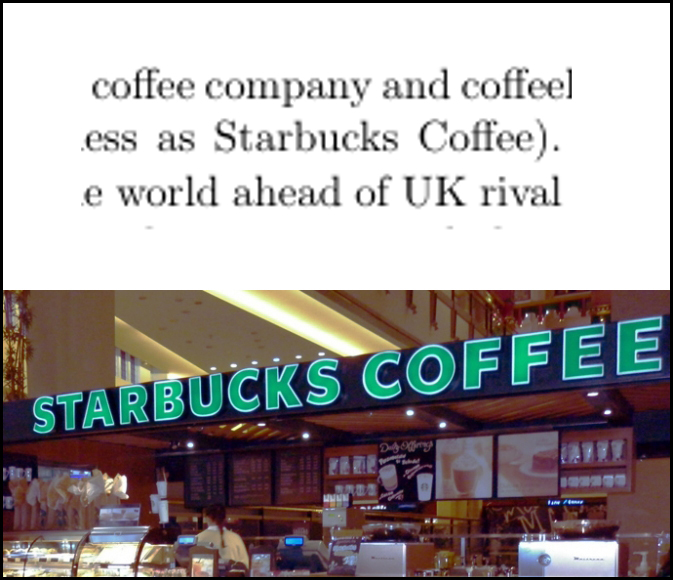
\includegraphics[scale=0.31]{img/ocr_vs_naturalImg_3.jpg}
				}
				\caption[OCRvsNaturales]{La parte superior muestra la imagen de un texto representada con una fuente de computadora donde se puede observar las palabras ``Starbucks Coffee''. La parte inferior expone las mismas palabras pero en una escena natural. Esto se realiza con el objetivo de observar las diferencias que hay entre analizar texto simple (fuente de computadora) y realizar el mismo trabajo en una imagen real}
				\label{fig: Optophone}
			\end{figure}
			
	En la literatura, uno de los esquemas de procesamiento más utilizados ha sido la detección de regiones dentro la imagen que corresponden a texto, su rectificación y la posterior aplicación de técnicas estándar de OCR (Kumar et al., 2007). Sin embargo, esta clase de técnicas se encuentra limitada a los escenarios en donde el OCR funciona correctamente, p.ej. en el reconocimiento de texto impreso (De Campos et al., 2009).

	Recientemente, se propuso un modelo (Wang et al., 2011) que emplea un esquema basado en técnicas de reconocimiento conocidas de la literatura de \textit{reconocimiento de objetos} (Navneet Dalal et al., 2005). En este caso, cada carácter alfanumérico se considera como un objeto a detectar y, empleando un conjunto de muestras de entrenamiento, se genera un modelo de clasificación mediante técnicas de aprendizaje supervisado (Christopher M. Bishop, 2007). Dada una nueva imagen, cada uno de estos clasificadores genera un conjunto de hipótesis sobre la presencia (y su ubicación) de cada símbolo alfanumérico en particular. Estas detecciones se utilizan luego en la detección de palabras específicas a partir de un léxico predefinido. Una particularidad del modelo propuesto por Wang et. al es la utilización de imágenes \textit{sintéticas} (generadas mediante simulación) en la generación de muestras de entrenamiento. Este enfoque reduce el problema de tener que recolectar una gran cantidad de imágenes naturales lo cual consume tiempo y esfuerzo. Mediante diferentes tipos de transformaciones, se busca crear un conjunto de imágenes de caracteres lo más parecido posible a uno real.
	
	
	\subsection{Sobre el trabajo}

	Esta tesis presenta una reimplementación de una sección del trabajo presentado por Wang et. al. en \cite{wang}. En dicha sección, los autores buscan establecer un método para poder reconocer caracteres en imágenes naturales. Para esto proponen usar un clasificador llamado \textit{Random Ferns} (se explica en detalle en el próximo capítulo) para lograr este objetivo.
	
	Este trabajo tiene como finalidad analizar la performance en el reconocimiento de caracteres en imágenes naturales de dicho clasificador. Esto se realiza a través de diferentes experimentos que buscan evaluar diferentes conjuntos de imágenes. El primero es usando imágenes reales, de la misma manera que Wang et. al., con lo cual se busca comparar ambas implementaciones. Posteriormente, se busca analizar como influyen los caracteres sintéticos o fuentes en diferentes proporciones. Estas se alteran con el objetivo de intentar imitar a las imágenes reales y ver si se puede alcanzar o superar los resultados del primer conjunto. Por último y a diferencia de los autores originales, se propone entrenar al clasificador con  un conjunto nuevo que surge de mezclar en diferentes proporciones imágenes reales y sintéticas.

	\subsection{Trabajos Relacionados}
	
	Se han propuesto muchos enfoques para afrontar el problema del reconocimiento de texto en imágenes naturales. De Campos et al. en \cite{dCBV09} comparan la performance de varios clasificadores (dentro de los cuales hay un motor de OCR comercial\footnote{http://abbyy.com/finereader}) sobre un dataset que ellos mismos crearon llamado \textit{Chars74K}. Sobre este dataset se corren varios experimentos del presente trabajo. Las conclusiones del trabajo destacan la dificultad que tienen los motores de OCR al momento de clasificar caracteres en imágenes naturales. Además, remarcan los beneficios de usar datos sintéticos para el entrenamiento los cuales logran un porcentaje de reconocimiento muy similar al obtenido con imágenes reales. También, realizan experimentos sobre un conjunto de imágenes de caracteres manuscritos. Sin embargo, no logran obtener buenos resultados en comparación con los otros experimentos. 
	
	Otro enfoque lo proponen B. Gatos et al. en \cite{GPP03}. El mismo consiste en una nueva metodología que ayuda a la detección, la segmentación y el reconocimiento automático de texto en imágenes naturales. Básicamente, la metodología consiste en lograr una eficiente binarización de las imágenes naturales. Para esto, dada una imagen natural, generan dos imágenes nuevas a partir de la original. La primera es una representación en escala de grises y la segunda es la versión invertida de la primera. Posteriormente, se les aplican diferentes técnicas para mejorarlas y así obtener la imagen binaria. Luego utilizan una función de decisión para elegir qué imagen contiene información de texto y a dicha imagen se le realiza un post-procesamiento para eliminar el ruido existente y mejorar su calidad. Después se realiza la detección de las áreas que contienen texto para poder utilizar finalmente el motor de OCR. Uno de los problemas que se desprenden de este enfoque es que al depender de un motor de OCR, el procesamiento que se realiza a la imagen tiene que ser muy bueno ya que la mayoría de las imágenes contienen ciertos defectos como una pobre iluminación, falta de foco, entre otros.

	L. Neumann y J. Matas \cite{LNJM} se diferencian de los enfoques tradicionales que constan en varias etapas de procesamiento y lo reemplazan con un marco de trabajo que consta de la verificación de hipótesis procesando de manera simultánea múltiples líneas de texto. Además, usan fuente de computadora como conjunto de entrenamiento.
	
	
	\subsection{Estructura de la Tesis}

	Esta tesis se desarrolla a lo largo de 5 capítulos.	
		
	En el capítulo 2 se procede a explicar los conceptos teóricos que involucran el presente trabajo. Principalmente se abordan los principios básicos del aprendizaje supervisado. Posteriormente se describen los conceptos necesarios para poder introducir  el clasificador Random Ferns. Finalmente, se realiza una introducción a las nociones básicas del procesamiento de imágenes.
	
	 En el capítulo 3, se describe el trabajo realizado por Wang et al. en \cite{wang} y se explica qué partes del mismo se han implementado en la presente tesis.

	En el capítulo 4, se abordan los experimentos realizados en el trabajo. Se describe tanto la implemetación del pipeline de procesamiento, como así también su diseño, el dataset usado y los resultados obtenidos. Por último se realiza un análisis completo de los resultados.
	
	En el último capítulo, de conclusiones y trabajos futuros, se hace un resumen de lo logrado a lo largo de esta tesis así como un descripción de los objetivos futuros que se pretenden seguir en este trabajo.

	
	%\subsection{Sobre Reconocimiento óptico de caracteres}

	\subsubsection{Definición del problema}
	
	El reconocimiento óptico de caracteres, usualmente abreviado OCR(por sus siglas en inglés), es la conversión mecánica o electrónica de imágenes escaneadas de texto impreso o mecanografiado en texto que pueda ser interpretado por una computadora. Es ampliamente utilizado como una forma de entrada de datos de algún tipo de fuente de datos original en papel, así sean documentos de pasaportes, facturas, extractos bancarios, recibos, tarjetas de visita, correo, o cualquier número de registros impresos\cite{arh-passport}\cite{arh-card}. Es un método común para la digitalización de textos impresos que pueden ser electrónicamente editados, buscados, almacenados de manera compacta, expuestos en linea y usados en procesos de máquinas como traducción de máquina, texto a voz, extracción de datos y minería de texto\cite{gbook}\cite{creaceed}. OCR es un campo de investigación en reconocimiento de patrones, inteligencia artificial y visión por computadora.
	
	\subsubsection{Aplicaciones}
		\begin{itemize}
			\item Reconocimiento automático de patentes\cite{arh-anpr}.
			\item Extraer información de una tarjeta de negocio a una lista de contacto \cite{x-root}.
			\item Hacer posible la búsqueda de imágenes electrónicas de documentos impresos. ej: \textit{Google Books} \cite{gbook}
			\item Convertir la escritura manual en tiempo real para controlar una computadora (\textit{pen computing})\cite{GKurt}\cite{sunnyside}.
			\item Tecnología de asistencia para usuarios ciegos y con deficiencias visuales \cite{creaceed}.
		\end{itemize}	
		
	\subsubsection{Componentes de un sistema OCR}
	
	A continuación se presentaran las diferentes etapas de un sistema OCR, como se puede apreciar en la figura \ref{fig: Sistema OCR}. Esta sección tiene como objetivo mostrar un panorama general de como funciona un sistema OCR, no tiene como objetivo adentrarse en detalles de implementación. En cada etapa se procederá a explicar brevemente cuales son las características importantes, haciendo incapié en la etapas de extracción de características y en la de clasificación y reconocimiento dado que son las etapas que se abordaron en este trabajo.
	
		\begin{figure}[htbp]
			\centering
			\fbox{ 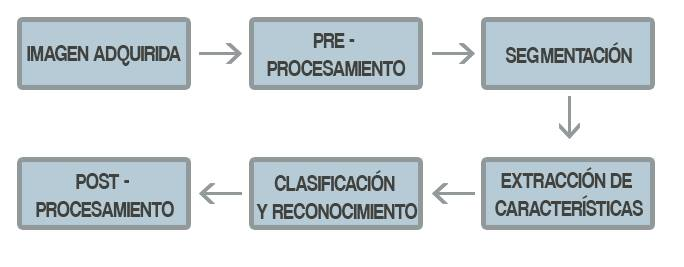
\includegraphics[scale=0.4]{img/OCR_pipeline_1.jpg} }
			\caption{Pipeline de un sistema OCR.}
			\label{fig: Sistema OCR}
		\end{figure}
	
		\paragraph{Pre-procesamiento} ~\\

		 El software de OCR aveces realiza un pre-procesamiento de las imágenes con el objetivo de tener más chances de un reconocimiento exitoso. Estas técnicas incluyen:
		  \begin{itemize}
		  	\item \textit{Enderezar} - Si el documento no está alineado debidamente cuando se escanea, puede necesitar posteriormente que se rote unos pocos grados en sentido horario o anti-horario con el objetivo de mantener el texto perfectamente vertical u horizontal \ref{fig: Enderezar}.
		  	\item \textit{Quitar manchas} - remover puntos negativos  y positivos, suavizar los bordes \ref{fig: Imagen con particulas} \ref{fig: Imagen suavizada}.
		  	\item \textit{Binarización} - Convertir la imagen de color o en escala de grises a blanco y negro (se llama "imagen binaria" justamente porque hay dos colores solamente). En algunos casos, esto es necesario para el algoritmo de reconocimiento de caracteres; en otros casos esta etapa se omite dado que el algoritmo tiene un mejor rendimiento con la imagen original \ref{fig: Binarizacion}.
		  	\item \textit{Eliminación de lineas} - Limpia las lineas y las cajas sin glifo \ref{fig: Eliminacion de lineas}.
		  	\item \textit{Análisis de disposición o "zoning"} - Identifica columnas, párrafos, títulos, etc. como bloques diferentes. Especialmente importante en tablas o disposiciones multi-columna \ref{fig: Zoning}.
		  	\item \textit{Detección de lineas y palabras} - Establece  la base para la forma del caracter y la palabra, separa las palabras si es necesario.
		  	\item \textit{Segmentación o aislación de caracter} - Múltiples caracteres que están conectados debido a artefactos de imagen deben ser separados; caracteres individuales que son separados en multiples piezas debido a artefactos deben ser conectados \ref{fig: Segmentacion}.
		  	\item \textit{Normalización de escala y relación de aspecto \ref{fig: Normalizacion y Suavizado}.}
		  \end{itemize}
		  
		\begin{figure}[htbp]
			\centering
			\subfloat[Imagen original torcida\label{fig: Imagen torcida}]{
				\fbox{ 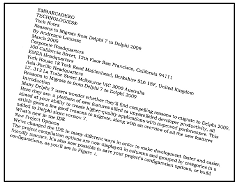
\includegraphics[scale=0.7]{img/skew_img.png} }
			}
			\subfloat[Imagen enderezada\label{fig: Imagen destorcida}]{
				\fbox{ 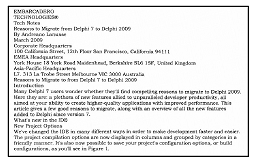
\includegraphics[scale=0.7]{img/deskew_img.png} }
			}
			\caption{Imagen enderezada}
			\label{fig: Enderezar}
		\end{figure}	
			  
		\begin{figure}[htbp]
			\centering
			\fbox{ 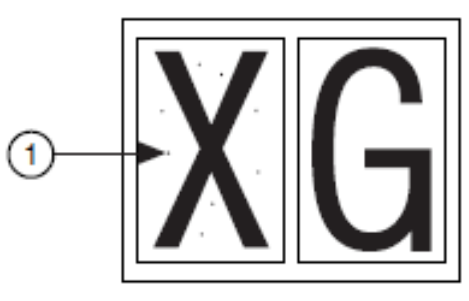
\includegraphics[scale=0.4]{img/rem_particles.png} }
			\caption[Imagen con partículas]{Comparación de caracteres con y sin partículas. 1. Imagen con partículas.}
			\label{fig: Imagen con particulas}
		\end{figure}
		
		\begin{figure}[htbp]
			\centering
			\fbox{ 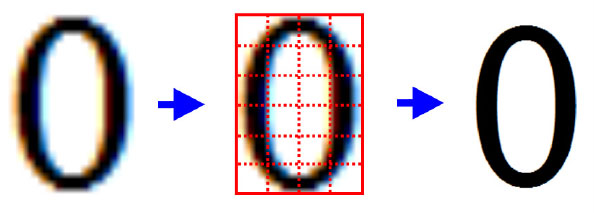
\includegraphics[scale=0.4]{img/smooth_char.png} }
			\caption{Imagen suavizada.}
			\label{fig: Imagen suavizada}
		\end{figure}
		
		\begin{figure}[htbp]
			\centering
			\subfloat[Imagen Original\label{fig: Imagen bin original}]{
				\fbox{ 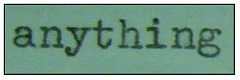
\includegraphics[scale=0.7]{img/bin_1.png} }
			}
			\subfloat[Imagen binarizada\label{fig: Imagen binarizada}]{
				\fbox{ 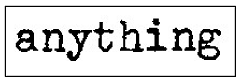
\includegraphics[scale=0.7]{img/bin_2.png} }
			}
			\caption{Binarización de una imagen}
			\label{fig: Binarizacion}
		\end{figure}
		
		\begin{figure}[htbp]
			\centering
			\subfloat[Imagen Original\label{fig: Imagen lines original}]{
				\fbox{ 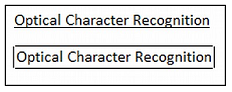
\includegraphics[scale=0.7]{img/lines_1.png} }
			}
			\subfloat[Imagen con las lineas removidas\label{fig: Imagen sin lineas}]{
				\fbox{ 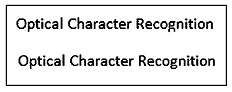
\includegraphics[scale=0.7]{img/lines_2.png} }
			}
			\caption{Eliminación de lineas}
			\label{fig: Eliminacion de lineas}
		\end{figure}
		
		\begin{figure}[htbp]
			\centering
			\fbox{ 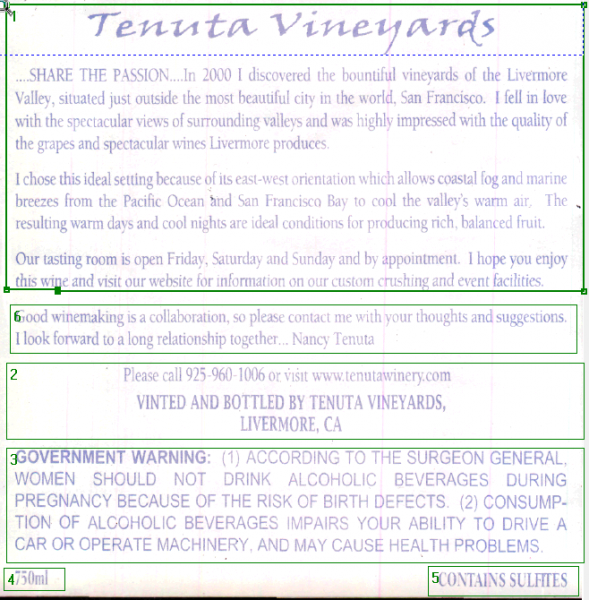
\includegraphics[scale=0.3]{img/zoning.png} }
			\caption{Análisis de disposición o "zoning".}
			\label{fig: Zoning}
		\end{figure}

		\begin{figure}[htbp]
			\centering
			\fbox{ 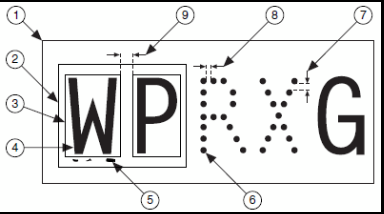
\includegraphics[scale=0.5]{img/segmentation.png} }
			\caption[Segmentación]{Segmentación. 1.Imagen Adquirida, 2.Región de interés, 3.Rectángulo del límite del carácter, 4.Carácter, 5.Artefacto, 6.Elemento, 7.Espaciado vertical, 8.Espaciado horizontal, 9.Espaciado del carácter.}
			\label{fig: Segmentacion}
		\end{figure}
		
		\begin{figure}[htbp]
			\centering
			\fbox{ 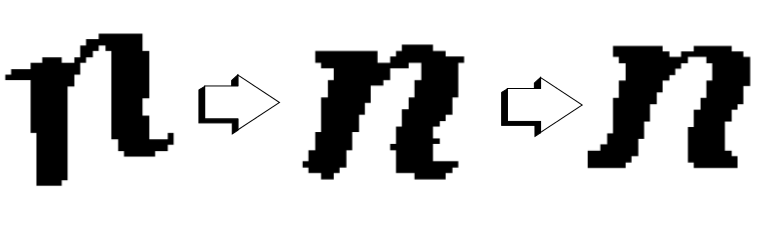
\includegraphics[scale=0.4]{img/norm_and_smoothing.png} }
			\caption{Normalización y suavizado de un símbolo.}
			\label{fig: Normalizacion y Suavizado}
		\end{figure}
	
\newpage
		\paragraph{Ubicación y segmentación}	 ~\\
		
		La segmentación es el proceso que determina los componentes de una imagen. Es necesario ubicar las regiones del documento donde se han impreso los datos y distinguirlos de los gráficos y las figuras. Por ejemplo, cuando se realiza el ordenamiento de correo automático, la dirección debe estar localizada y separada de otras impresiones en el sobre como las estampillas o logos de empresa, anterior al reconocimiento.
		
		Aplicado al texto, la segmentación es la aislación de caracteres o palabras. La mayoría de los algoritmos de reconocimiento óptico de caracteres segmentan las palabras en caracteres aislados los cuales son reconocidos individualmente. Usualmente esta segmentación es realizada aislando cada componente conectado, es decir, cada área negra conectada. Esta técnica es fácil de aplicar, pero los problemas ocurren si los caracteres se tocan o si los caracteres están fragmentados y consisten de varias partes, si el texto tiene mucho ruido o se confunde con alguna imagen, entre otros. ~\ref{fig: Caracter quebrado}~\ref{fig: Caracteres unidos 1}~\ref{fig: Caracteres unidos 2}~\ref{fig: Caracteres en graffiti}~\ref{fig: Captcha}.

		\begin{figure}[htbp]
			\begin{minipage}{.3\linewidth}
				\centering
				\subfloat[Captcha\label{fig: Captcha}]{
					\fbox{ 
\includegraphics[scale=0.2]{img/degraded_1.jpg} }
				}
			\end{minipage}
			\begin{minipage}{.3\linewidth}
				\centering
				\subfloat[Carácter quebrado\label{fig: Caracter quebrado}]{
					\fbox{ 
\includegraphics[scale=0.3]{img/degraded_2.jpg} }
				}
			\end{minipage}
			\begin{minipage}{.3\linewidth}
				\centering
				\subfloat[Caracteres unidos por la tipografía\label{fig: Caracteres unidos 1}]{
					\fbox{ 
\includegraphics[scale=0.3]{img/degraded_3.jpg} }
				}
			\end{minipage}
			\begin{minipage}{.3\linewidth}
				\centering
				\subfloat[Carácter con linea superpuesta\label{fig: Caracter y linea}]{
					\fbox{ 
\includegraphics[scale=0.3]{img/degraded_4.jpg} }
				}
			\end{minipage}
			\begin{minipage}{.3\linewidth}
				\centering
				\subfloat[Caracteres unidos\label{fig: Caracteres unidos 2}]{
					\fbox{ 
\includegraphics[scale=0.3]{img/degraded_5.jpg} }
				}
			\end{minipage}
			\begin{minipage}{.3\linewidth}
				\centering
				\subfloat[Un graffiti como el de la imagen puede hacer pasar el texto como imagen.\label{fig: Caracteres en graffiti}]{
					\fbox{ 
\includegraphics[scale=0.2]{img/text_like_graphic.jpg} }
				}
			\end{minipage}
			\caption{Problemas de segmentación}
			\label{fig: Problemas de segmentacion}
		\end{figure}
		
	
		\paragraph{Extracción de características} ~\\
		
		El objetivo de la extracción de características es capturar los rasgos esenciales de los caracteres para formar vectores de características y es generalmente aceptado como uno de los problemas más difíciles en el reconocimiento de patrones. Se vuelve sencillo para el clasificador el clasificar entre clases diferentes teniendo en cuenta estas características \cite{PSH2011}. Acorde al trabajo de C. Y. Suen \cite{Suen86}, los rasgos de un carácter pueden ser clasificados en dos clases: características globales o estadísticas y características estructurales o topológicas.
		\begin{itemize}
			\item \textbf{Características globales o estadísticas}. \\
				Las características globales son obtenidas del arreglo de puntos que constituyen la matriz del carácter. Estas características pueden ser detectadas fácilmente en comparación con las características topológicas. Además no son afectadas demasiado por el ruido o la distorción en comparación a las topológicas. Un número de técnicas se utilizan para lograr la extración de características, estas son: \textit{momentos, zonificación, histogramas de proyección, n-tuplas y cruce y distancias}
				\begin{itemize}
					\item \textbf{Momentos}
					En este caso los diferentes puntos presentes en un carácter son utilizados como características. Heutte et al. \cite{Heutte98} decían que estos métodos son más comúnmente usados en el reconocimiento de caracteres.
					\item \textbf{Zonificación}
					De acuerdo con esta técnica, la matriz del carácter es dividida en pequeñas porciones o zonas. Las densidades de los píxeles en cada zona son calculadas y usadas como características. Este concepto fue sugerido por Hussain et al.\cite{Hussain72}.
					\item \textbf{Histogramas de proyección}
					Los histogramas de proyección nos da el número de píxeles negros en las direcciones horizontal y vertical de un área específica del carácter. El concepto fue introducido por M. H. Glauberman \cite{Glauberman56}. Los histogramas de proyección pueden ser vertical, horizontal, diagonal izquierda o derecha.
					\item \textbf{N-tuplas}
					De acuerdo con este método, la posición de los píxeles blancos o negros en la imagen de un carácter es considerado una característica. El método fue desarrollado por Tarling y Rohwer \cite{TR93}.
				\end{itemize}
			\item \textbf{Características estructurales o topológicas}. \\
				Estas características están relacionadas con la geometría del conjunto de caracteres. Algunas de estas características son concavidades y convexidades en los caracteres, el número de puntos finales, el número de agujeros en los caracteres, etc. Muchas investigaciones fueron realizadas con el objetivo de encontrar diferentes características estructurales.
				
				Rocha y Pavlidis \cite{RP94} propusieron un método para el reconocimiento de caracteres impresos del tipo multi-fuente. Para este método se han utilizado características estructurales tales como puntos singulares, arcos convexos y trazos.
				
				Otro método similar fue propuesto por A. Amin \cite{Amin2000}. Aquí se han usado características estructurales como el número de subpalabras, el número de picos en cada subpalabra, el número de curvas de cada pico, entre otros.
				
		\end{itemize}
		  
		  	En el presente trabajo, las características de una imagen son representadas por un vector binario que se obtiene de binarizar el descriptor HOG(concepto descripto en la sección \ref{sec: HOG}) de dicha imagen con un umbral pre-calculado. Este método de extracción de características se abordará más adelante en el capítulo 4 cuando se explique el pipeline de procesamiento.
	  
		\paragraph{Clasificación y Reconocimiento} ~\\
		
		La clasificación es el proceso de identificar cada carácter y asignarle la clase correcta. La clasificación se hace generalmente mediante la comparación de los vectores de características que corresponden al carácter de entrada con el representante de cada clase de carácter. Pero antes de hacer esto, el clasificador debe entrenarse con un conjunto de entrenamiento que represente a las diferentes clases de caracteres. Varios investigadores han propuesto métodos de clasificación dentro de los cuales se encuentran los métodos estadísticos, métodos sintácticos, comparación de plantillas, redes neuronales artificiales, métodos de núcleo~\cite{NNSJ}~\cite{SA96}~\cite{RYVY2010}.
		
		Como se procederá a explicar en detalle en el capítulo 3, el clasificador que se usa en este trabajo es Random Ferns. Las razones de su elección se basan en que es un clasificador multi-clase bastante eficiente y dado que el problema en cuestión es clasificar caracteres (representan 62 clases en total), su elección resulta apropiada.
		
		El aporte de este trabajo se basa en analizar la performance del clasificador Random Ferns cuando es entrenado con caracteres sintéticos. Si bien este enfoque fue abordado en \cite{wang}, en dicho trabajo no se puede apreciar como influye en la clasificación la cantidad de imágenes sintéticas usadas al entrenar el clasificador. En su trabajo, hacen uso de 1000 imágenes sintéticas por clase para entrenar el clasificador y realizan una comparación de performance entre el entrenamiento con imágenes sintéticas y el realizado con imágenes reales. Este trabajo va un paso más allá y busca ver si el número de imágenes sintéticas por clase influye realmente en la performance y además se busca analizar un nuevo enfoque en el cual se mezclan en diferentes proporciones imágenes reales con sintéticas para observar que tan efectivo resulta ser el clasificador en esas condiciones.
		
		\paragraph{Post-procesamiento} ~\\
		
		La precisión de OCR puede ser incrementada si la salida está restringida por un lexicón, que es una lista de palabras cuya aparición está permitida dentro del documento. Este puede ser, por ejemplo, todas las palabras del lenguaje español, o un lexicón mas técnico para un campo en particular. Esta técnica puede ser problematica si el documento contiene palabras que no están en el lexicón, como nombres propios.
		
		La salida puede ser texto plano o un archivo de caracteres, pero sistemas de OCR más sofisticados pueden conservar la disposición original de la pagina y producir, por ejemplo, un PDF con anotaciones que incluyan la imagen original de la página y una representación textual de búsqueda.
		
		Conocer la gramática del lenguaje que está siendo escaneado puede ayudar a determinar si la palabra es un verbo o un sustantivo, por ejemplo, permitiendo una gran precisión.
		
	\subsubsection{Errores típicos en OCR}
	
		La precisión de los sistemas de OCR es, en la práctica, directamente dependiente de la calidad de los documentos de entrada. Las principales dificultades se pueden clasificar como sigue:
		\begin{itemize}
			\item \textit{Variaciones en la forma}, debido a las variaciones en el estilo y los remates o serifas.
			\item \textit{Deformaciones}, causados por caracteres quebrados, manchados y moteados.
			\item \textit{Variación en el espaciado}, debido a los superíndices, subíndices, sesgo y la variable de espaciado.
			\item \textit{Mezcla de texto e imágenes}.
		\end{itemize}
		Estas imperfeccciones pueden afectar y ocasionar problemas las diferentes etapas del proceso de reconocimiento de un sistema OCR, resultando en errores de clasificación y rechazos.	
	
		

	
	%	\newpage
	\subsection{Repercusión social del tema}
		\label{sec:repercusion_social}
		Cheap brainstorm:
		\begin{itemize}
		 \item digitalizar documentos
		 \item brindar mejor calidad de  vida a gente con discapacidades
		 
		\end{itemize}




	\newpage	
\section{Marco teórico}

	\subsection{Aprendizaje automático}

	Desde la máquina construida por Blaise Pascal en 1642 para realizar sumas, la primera computadora programable electrónica ENIAC, hasta la actualidad, el hombre siempre ha demostrado interés por automatizar ciertos procesos. En particular, el tener una máquina que pudiera leer como una persona era un sueño, que tuvo sus inicios alrededor de 1914 cuando Edmund Fournier d'Albe desarrolló el \textit{Optophone} (ver Figura \ref{fig: Optophone}), que era un escáner de mano que al moverlo a través de una página impresa, producía tonos que correspondían	a letras o caracteres específicos \cite{EFdAlbe}.

			\begin{figure}[htbp]
				\centering
				\centerline{
					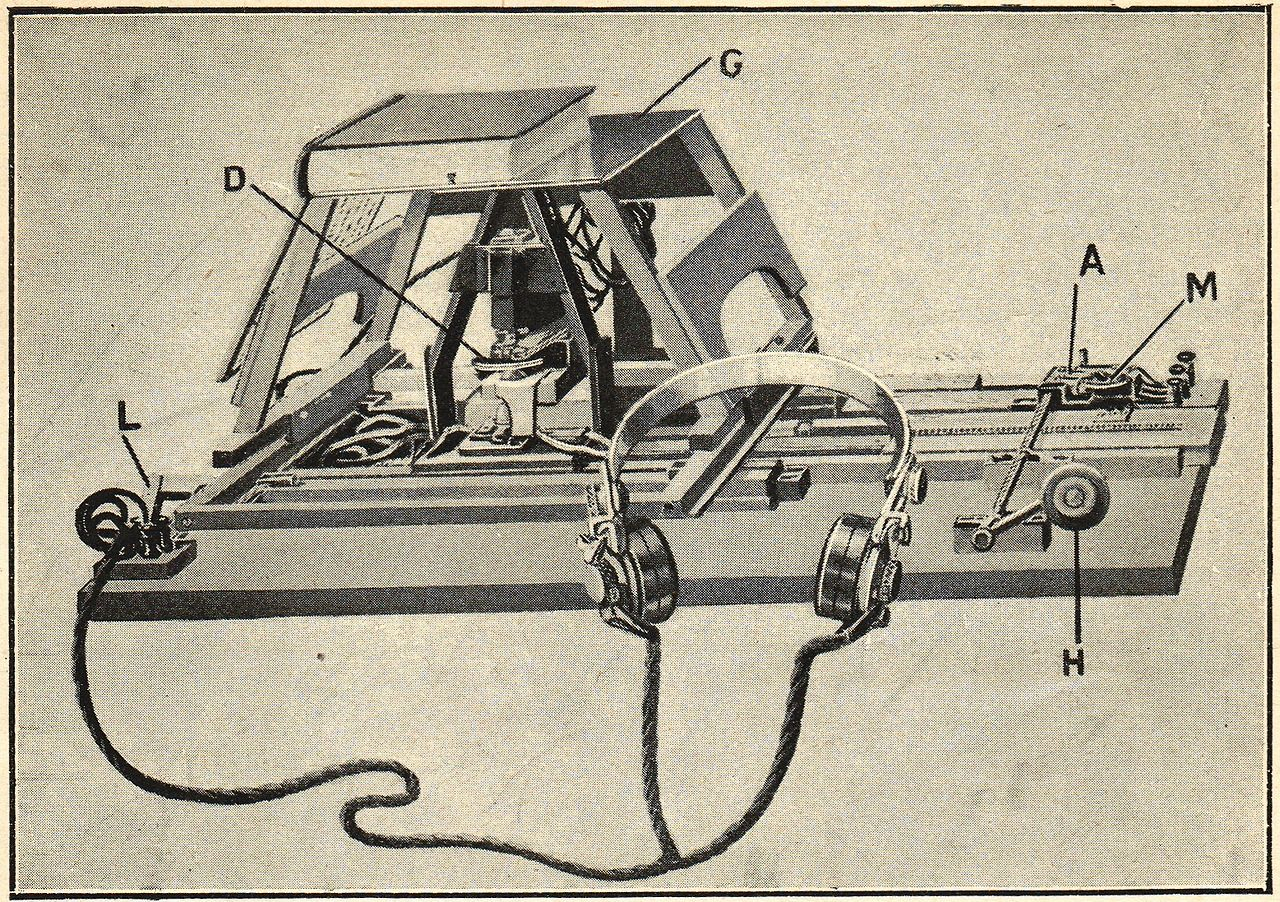
\includegraphics[scale=1]{img/Optophone.jpg}
				}
				\caption[Optophone]{Imagen del \textit{Optophone} en detalle. Extraida de la revista Vetenskapen och livet (1922).}
				\label{fig: Optophone}
			\end{figure}
			
	Durante gran parte del siglo \rom{20} y hasta el día de hoy, la cantidad de información almacenada en libros y documentos escritos ha crecido de manera exponencial. Esto se debe a que cada día se vive en un mundo más glo\-ba\-li\-za\-do, donde la información es una herramienta fundamental en cualquier ámbito. Con el surgimiento de las primeras computadoras y la digitalización de la información, se volvió más fácil compartir datos. Sin embargo, el proceso de digitalizar los documentos ya existentes era un proceso tedioso ya que se hacía manualmente. Era imperativo tener métodos automáticos que ayudaran a clasificar y analizar toda esa información. Dada esta necesidad es que surge el campo del \textit{aprendizaje automático} o \textit{machine learning} que, en palabras de K. P. Murphy \cite{Murphy12}, estudia métodos que permiten detectar automáticamente patrones en los datos y luego usar esos patrones descubiertos para predecir datos futuros o poder tomar ciertas decisiones en condiciones de incertidumbre. 
	
	Uno de los temas que se tratan en este campo es el del reconocimiento de texto en imágenes. Las aplicaciones son muy numerosas, desde ayudar a las personas no videntes, \cite{Optelec}, realizar detección de patentes de automóviles, \cite{DAB}, o hacer traducción automática de textos en diferentes idiomas \cite{WordLens}.
	 
	 El campo del \textit{aprendizaje automático} tiene fuertes bases en la estadística por lo cual, los conceptos como los desarrollados en el apéndice \ref{section:Apendice-A} van a ser de utilidad para comprender las siguientes subsecciones.
	 
	 De todas las técnicas existentes en este campo, las que se van a ver a continuación son la de: aprendizaje supervisado y no supervisado.
	 	
	\subsubsection{Aprendizaje supervisado}
	
	Como manifiesta Murphy, el aprendizaje supervisado es una técnica del aprendizaje automático cuyo objetivo es, dado un conjunto de entrada $X$ y uno de salida $Y$, establecer un mapeo entre $X$ e $Y$ dado un conjunto etiquetado de pares de entrada-salida $M=\{(x_i,y_i) x_i \in X, y_i \in Y \}^{N}_{i=1}$ donde $M$ es llamado el \textit{conjunto de entrenamiento} y $N$ es el número de ejemplos de entrenamiento \cite{Murphy12}.
	
	El conjunto de entrenamiento es un elemento indispensable en cualquier algoritmo de aprendizaje supervisado, ya que representa la base fundamental de conocimiento necesaria para que el algoritmo pueda realizar futuras predicciones. En general, mientras más conocimiento se tenga sobre las ca\-rac\-te\-rís\-ti\-cas del objeto de interés que se esté analizando, más precisa va a ser la clasificación sobre nuevas entradas. Esto último hace referencia al concepto de \textit{generalización}. Como expresa M. Mohri et. al. en \cite{MMohri}, es la habilidad de interpretar con precisión nuevas entradas luego de haber ``experimentado'' un conjunto de entrenamiento. Este conocimiento se construye a partir de la variabilidad de los objetos conocidos, es decir el poder contar con un gran conjunto de muestras que reflejen las posibles variaciones del objeto de interés. Esto le otorga robustez a la clasificación. Por ejemplo, con\-si\-de\-re\-mos un clasificador de caracteres alfanuméricos que tiene como conjunto de entrenamiento un grupo de imágenes que representan a cada carácter individualmente. Luego, dado que un carácter puede estar representado de diferentes formas, es decir, pueden haber variaciones en la perspectiva del mismo, en la iluminación del ambiente, el ruido de la imagen, entre otros, es necesario poder contar con la mayor cantidad de estas variaciones. Esto se debe a que mientras más conocimiento se tenga sobre las características del objeto de interés y las diferentes formas en que este puede aparecer, más certera va a ser la clasificación sobre nuevas entradas. Esto es lógico pues las nuevas entradas van a ser variaciones de los elementos que tenemos en el conjunto de entrenamiento.
	
	Murphy dice que en la configuración más simple, cada entrada $x_i$ del conjunto de entrenamiento es un vector $D$-dimensional de números. Estas son llamadas \textit{características} (\textit{features}, de su traducción al inglés). En general, sin embargo, $x_i$ puede ser un objeto con una estructura compleja, como una imagen, un mensaje de correo, etc.
	
	El autor destaca que, dependiendo del tipo de problema a tratar, la salida $y_i$ puede ser una variable categórica, donde $y_i \in \{1,\dots,C\}$ (conjunto finito de clases), o puede ser un valor real. Cuando $y_i$ es una variable categórica, estamos frente a un problema de \textit{clasificación} donde el objetivo es ``etiquetar'' o nombrar los objetos observados. Cuando $y_i$ es una variable real, estamos en presencia de un problema de regresión, que es similar a la clasificación excepto que la respuesta es en general una variable continua.	
	

	\subsubsection{Aprendizaje no supervisado}
	
		En \cite{Murphy12}, se describe al aprendizaje no supervisado como una técnica del aprendizaje automático cuyo objetivo es encontrar ``estructuras interesantes'' en los datos. Murphy resalta que, a diferencia del aprendizaje supervisado, no se establece qué salida se tiene que dar para cada entrada. En cambio, se busca construir modelos de la forma $p(x_i | \theta)$ donde $\theta$ es un vector de parámetros y $x_i$ es un dato de entrada. La diferencia con el aprendizaje supervisado, es que hemos establecido $p(x_i | \theta)$ en vez de $p(x_i | y_i, \theta)$; es decir, el aprendizaje supervisado es una estimación condicional en la variable de interés, mientras que el aprendizaje no supervisado es una estimación no condicional.
		
		Según el autor, el aprendizaje no supervisado no requiere que haya una persona que etiquete los datos manualmente. No solo es costoso, sino que además contiene relativamente poca información, sin duda no es suficiente para estimar de forma fiable los parámetros en modelos más complejos.
	
	\subsection{Clasificación}

		Como explica de manera sencilla Murphy K. P. en \cite{Murphy12}, el objetivo del aprendizaje supervisado es aprender un mapeo desde las entradas $x$ a las salidas $y$. En clasificación, $y_i \in \{1,\dots,C\}$ con $C$ siendo el número de clases. Si $C=2$, estamos frente al problema de \textit{clasificación binaria}; mientras que si $C>2$, la clasificación pasa a ser \textit{multiclase}. Existe otro tipo de clasificación denominada \textit{clasificación multi-etiqueta}, que difiere de la multiclase en cuanto a que las clases no son mutuamente excluyentes, es decir, una muestra puede pertenecer a dos o más categorías o clases. En este último caso, el mapeo se realiza desde la entrada $x$ a un vector $z$, más que a una salida escalar. La elección de cual usar esta directamente asociada al tipo de problema que se quiera resolver.
		
		Tal como expresa P. Domingos en \cite{PDomingo}, el objetivo del aprendizaje automático es \textit{generalizar} más allá de los ejemplos en el conjunto de entrenamiento. Ya que, no importa cuantos datos tengamos, es muy poco probable que vayamos a ver los mismos ejemplos al momento de evaluar.
		
		Para Murphy, una manera de formalizar el problema es a partir de una función de aproximación. Se asume $y = f_{\theta}(x)$ para cierta función desconocida $f_{\theta}$, y el objetivo del aprendizaje es estimar los parámetros $\theta$ de la función $f$ dado un conjunto de entrenamiento etiquetado. Posteriormente, se realizan predicciones usando $\hat{y} = f_{\hat{\theta}}(x)$ (usamos el símbolo \string^ para denotar estimación). El objetivo principal es realizar predicciones en entradas nuevas, es decir, que no se hayan visto durante el entrenamiento.
		
		Como se habrá podido observar hasta acá, la clasificación es un tema de gran relevancia en el aprendizaje automático. Hacer que un programa aprenda en base a ejemplos y pueda posteriormente reconocer elementos similares es un gran desafío. Por eso es importante encontrar la mejor forma de entrenar a estos programas también denominados clasificadores.
		
		En la próxima subsección, se va a realizar una introducción a los clasificadores probabilísticos y a la teoría de decisión. También, se presentaran varios clasificadores importantes para la comprensión del presente trabajo como Na\"{i}ve Bayes, Random Forest y Random Ferns, siendo los dos primeros de relevancia para comprender al último.
		
		
	\subsubsection{Clasificadores Probabilísticos}

		Los clasificadores probabilísticos determinan, dada una entrada nueva, la probabilidad de que esta pertenezca a un conjunto de clases, a diferencia de otros clasificadores, que simplemente predicen a que clase pertenece la misma. Esto lo realiza asignando una distribución de probabilidad al conjunto de clases.
	
	Formalmente un clasificador probabilístico es una distribución condicional $p(Y|X)$ sobre un conjunto finito de clases $Y$ dada $X$ entradas. Una forma de determinar cual es la mejor clase $\hat{y} \in Y$ para $X$ sería elegir la clase con la probabilidad más alta
	$$\hat{y} = argmax_{y}p(Y=y|X) $$
	
	Uno de los clasificadores más populares es \textit{na\"{i}ve Bayes} (que se procede a explicar en las próximas secciones). Este clasificador junto con el resto, derivan de modelos de probabilidad generativos que proporcionan un principio para el estudio de la clasificación estadística en dominios complejos tales como el lenguaje natural y el procesamiento visual \cite{GargRo01}.


	%\subsubsection{Teoría de decisión}
	
	La teoría de decisión nos ayuda a tomar decisiones óptimas en situaciones que involucran incertidumbre. La incertidumbre hace referencia a un estado de conocimiento limitado donde es imposible describir con exactitud el estado existente, la salida futura, o más de una posible salida.
	
	Supongamos que tenemos un vector $x$ como entrada junto con el correspondiente vector $t$ de variables objetivo, la meta es predecir $t$ dado un nuevo valor de $x$. En problemas de regresión, $t$ comprenderá variables continuas, mientras que en problemas de clasificación $t$ representará etiquetas de clase. La determinación de la probabilidad conjunta de $x$, $t$ denotada como $p(x,t)$ dado un conjunto de datos de entrenamiento es un ejemplo de \textit{inferencia} y es típicamente un problema muy difícil. La inferencia, en este caso, hace relación a la estadística inferencial la cual es una parte de la estadística que comprende los métodos y procedimientos que por medio de la inducción determina propiedades de una población estadística, a partir de una pequeña parte de la misma.
	
	Consideremos el siguiente ejemplo, sea $C=\{C_1,\dots,C_k\}$ un conjunto de etiquetas de clase, sea $t \in C$ y sea $x$ un vector de entrada nuevo. Se desea determinar a que clase pertenece $x$. El problema de inferencia involucra determinar la distribución conjunta $p(x,C_k)$, o equivalentemente $p(x,t)$.

	Como se dijo anteriormente, el objetivo es decidir a cual de las $k$ clases pertence el vector de entrada $x$ . Estamos interesados entonces, en las probabilidades de las $k$ clases dado $x$, es decir $p(C_k|x)$, $k=1,\dots,K$. Usando el Teorema de Bayes, estas probabilidades pueden expresarse de la forma:
		\begin{align*}
			p(C_k|x) = \frac{p(x|C_k)p(C_k)}{p(x)}
		\end{align*}

	Ahora podemos interpretar $p(C_k)$ como la probabilidad a priori para la clase $C_k$, y $p(C_k|x)$ como la correspondiente probabilidad a posteriori. Por ejemplo, $p(C_1)$ representa la probabilidad de pertenecer a la clase $C_1$, antes de observar la muestra $x$
	
	Se pueden distinguir dos etapas en el problema de clasificación, la \textit{etapa de inferencia} en el cual se usan los datos para entrenar el modelo para $p(C_k|x)$, y la subsecuente \textit{etapa de decisión} en la cual se usan las probabilidades a posteriori para poder realizar asignaciones óptimas de las clases. Una alternativa, es la de resolver ambos problemas en conjunto y simplemente entrenar una función que mapee las entradas $x$ directamente con las decisiones. Dicha función es llamada \textit{función discriminante}.
	
	De hecho, se pueden identificar tres enfoques diferentes al momento de resolver problemas de decisión. En orden decreciente de complejidad, estos son:
		\begin{enumerate}
			\item Primero, resolver el problema para determinar las densidades condicionales $p(x \vert C_k)$ para cada clase $C_k$ individualmente. También de forma separada, inferir las probabilidades de clases a priori $p(C_k)$. Después, usar el teorema de Bayes en la forma:
			$$p(C_k \vert x) = \frac{p(x \vert C_k)p(C_k)}{p(x)} $$
			para encontrar las probabilidades a posteriori $p(C_k \vert x)$. Como es usual, el denominador en el teorema de Bayes puede ser encontrado en término de las cantidades que aparecen en el numerador, como:
			 $$p(x) = \sum_k p(x \vert C_k)p(C_k) $$
			Equivalentemente, se puede modelar la distribución conjunta $p(x,C_k)$ directamente y después normalizar para obtener las probabilidades a priori. Habiendo encontrado las probabilidades a posteriori, se puede usar la teoría de decisión para determinar la pertenencia a una clase para cada entrada nueva $x$. Los enfoques que explícitamente o implícitamente modelan la distribución de las entradas así también como las salidas son conocidos como \textit{modelos generativos}, debido a que tomando muestras de ellos es posible generar puntos de datos sintéticos en el espacio de entrada.
			\item Primero, resolver el problema de inferencia para determinar las  probabilidades de clase a posteriori $p(C_k \vert x)$, y luego subsecuentemente usar la teoría de decisión para asignar a cada $x$ nueva una de estas clases. Los enfoques que modelan las probabilidades a posteriori directas son llamados \textit{modelos discriminativos}.
			\item Encontrar una función $f(x)$, llamada función discriminante, que mapea directamente cada entrada $x$ con una etiqueta de clase. Por ejemplo, en el caso del problema de dos clases, $f(\cdot)$ puede ser valuada de manera binaria, de manera que $f = 0$ represente a la clase $C_1$ y $f = 1$ represente a la clase $C_2$. En este caso, las probabilidades no toman partido. 
		\end{enumerate}
		
	Consideremos los méritos relativos a estas tres alternativas. El enfoque (1) es el más demandante debido a que involucra encontrar la distribución conjunta tanto de $x$ como de $C_k$. Para muchas aplicaciones, $x$ tendrá alta dimensionalidad, y por consiguiente puede ser necesario un conjunto de entrenamiento grande con el fin de ser capaz de determinar las densidades de clase condicional con una exactitud razonable. Hay que tener en cuenta que la probabilidades a prior $p(C_k)$ de la clase a menudo pueden estimarse simplemente a partir de las proporciones de los punto de datos del conjunto de entrenamiento en cada una de las clases.
		
	Sin embargo, si sólo deseamos realizar decisiones de clasificación, esto conlleva a un gasto de recursos computacionales y una demanda de datos excesiva para encontrar la distribución conjunta $p(x, C_k)$ cuando de hecho, solamente se necesitan las probabilidades a posteriori $p(C_k \vert x)$, las cuales pueden ser obtenidas a través del enfoque (2). 
		
	Un enfoque mucho más simple es (3) en el cual se usa una conjunto de entrenamiento para encontrar una función discriminante $f(x)$ que mapea cada $x$ directamente a una etiqueta de clase, así combinando la inferencia y las etapas de decisión en un simple problema de aprendizaje.
		
	Con la opción (c), sin embargo, se pierde el acceso a las probabilidades a porteriori $p(C_k \vert x)$. 
	
	\subsubsection{Vectores de características} \label{subsec:feature}

	Un característica o feature, es un aspecto o cualidad distintiva de un objeto (clase de interés). Las características son importantes dado que al representar los aspectos o cualidades mas significativas de un objeto, facilitan el reconocimiento posterior de objetos similares. Esto es fundamental por ejemplo, en los esquemas de clasificación en el aprendizaje supervisado ya que permite, dada una muestra desconocida, identificar a que clase pertenece si anteriormente sabemos las características particulares de cada clase (a partir de instancias o muestras analizadas con anterioridad). Esto conlleva a que si se realiza una buena selección de características, impacte positivamente en la precisión de los clasificadores y por ende en el reconocimiento. Por ejemplo, en los algoritmos de detección de spam, las características pueden incluir el lenguaje en el que esta escrito el email, la ausencia o presencia de ciertos encabezados, la corrección gramatical del texto, entre otros~\cite{SpamPaper}.

	Un vector de características o ``feature vector'', es un  vector $n$-dimensional de características numéricas que se diseña de forma tal de conjeturar propiedades características de los objetos. Muchos algoritmos en machine learning requieren la representación numérica de los objetos, dado que dichas representaciones facilitan el análisis estadístico y el procesamiento de los datos.
		
	
		
	

	
	\subsubsection{Clasificador Na\"{i}ve Bayes}

	Es un clasificador probabilístico basado en la aplicación del teorema de Bayes con una fuerte suposición de independencia (na\"{i}ve). En términos simples, un clasificador na\"{i}ve Bayes asume que la presencia o ausencia de una característica particular no está relacionada con la presencia o ausencia de cualquier otra característica. Este tipo de clasificador considera que cada una de estas características contribuye independientemente a la probabilidad de que un elemento sea de una clase particular, independientemente de la presencia o ausencia de otras características. Por ejemplo, una fruta puede ser considerada una manzana si es roja, redonda y de 7cm de diámetro aproximadamente.

	El modelo para un clasificador es:
		$$p(C \vert F_1,\dots,F_n)$$
	sobre una variable dependiente C, con un pequeño número de resultados (o clases). Esta variable está condicionada por varias variables independientes (\textit{features}) desde $F_1$ a $F_n$. El problema es que si el número $n$ de variables independientes es grande (o cuando éstas pueden tomar muchos valores), entonces basar este modelo en tablas de probabilidad se vuelve computacionalmente imposible ya que, por ejemplo, si hubiesen $35$ variables independientes con $2$ valores posibles cada una entonces habrían $34.359.738.368$ valores posibles distribuidos en múltiples tablas. Si se usaran decimales de punto flotante simple (4 bytes), se necesitarían 32 gigabytes de memoria para almacenar todo, lo que lo hace muy poco manipulable. Por lo tanto el modelo se reformula para hacerlo más manejable:
Usando el teorema de Bayes se escribe:
		\begin{align*}
		p(C \vert F_1,\dots,F_n) = \frac{p(C) \ p(F_1,\dots,F_n\vert C)}{p(F_1,\dots,F_n)}.
		\end{align*}
		que puede ser reescrita como sigue, aplicando repetidamente la definición de probabilidad condicional:
		\begin{align}
		p(C, F_1, \dots, F_n)
		&= p(C) \ p(F_1,\dots,F_n\vert C) \\
		&= p(C) \ p(F_1\vert C) \ p(F_2,\dots,F_n\vert C, F_1) \\
		&= p(C) \ p(F_1\vert C) \ p(F_2\vert C, F_1) \ p(F_3,\dots,F_n\vert C, F_1, F_2)
		\end{align}
		y así sucesivamente. Ahora es cuando la asunción "na\"{i}ve" de independencia condicional entra en juego: se asume que cada $F_i$ es independiente de cualquier otra $F_j$ para $j \neq i$. Esto significa que
		\begin{align*}
		p(F_i \vert C, F_j) = p(F_i \vert C)
		\end{align*}
		por lo que la probabilidad compuesta puede expresarse como
		\begin{align*}
		p(C, F_1, \dots, F_n) 
		&= p(C) \ p(F_1\vert C) \ p(F_2\vert C) \ p(F_3\vert C) \dots \\
		&= p(C) \prod_{i=1}^n p(F_i \vert C).
		\end{align*}
		Esto significa que haciendo estas presunciones, la distribución condicional sobre C puede expresarse de la siguiente manera:
		$$p(C \vert F_1,\dots,F_n) = \frac{1}{Z}p(C)\prod_{i=1}^n p(F_i \vert C)$$
		donde $Z$ es un factor que depende sólo de $F_1,\dots , F_n$, es decir, constante si los valores de $F_i$ son conocidos.
		
	
	\subsubsection{Árboles de decisión}
\label{subsection:arboles_decision}

%	Desde el punto de vista de las ciencias de la computación y las matemáticas, un árbol es un grafo conexo simple y sin ciclos, y sus propiedades son básicas de la teoría de grafos. Formalmente, un grafo es una estructura de la forma $G=(V,E)$, donde $V$ es un conjunto de vértices o nodos y $E=\{ (v_i, v_j), v_j,v_i \in V \}$ es un conjunto de pares donde cada par representa una arista o rama que conecta a dos nodos.

%	Además, definimos un \textit{camino} o \textit{path} entre los nodos $v_i, v_j \in V, i \neq j$ en $G$ (lo denotamos $P_{v_i, v_j}^G$), como el conjunto $\{ v_i, v_{i+1}, \dots, v_{j-1}, v_j \}$ de nodos talque  $(v_k, v_{k+1}) \in E, k = i, \dots, (j-1)$. Luego, decimos que $G$ es conexo si $\forall v_i, v_j \in V, i \neq j, \exists P_{v_i, v_j}^G$ y no tiene ciclos si $\forall v_i, v_j \in V, i \neq j, \exists ! P_{v_i, v_j}^G $.

	%En un árbol existen dos tipos de nodos. La diferencia radica en la cantidad de nodos adyacente al mismo o grado del nodo, que se denota como $d(v_i), v_i \in V$. Los nodos con grado $\leq 1$ se denominan hojas y el resto son nodos internos. Los árboles que se consideran en este trabajo tienen un tercer tipo de nodo que llamamos raíz y es único. Los árboles con raíz son muy comunes en el área de aprendizaje automático y formalmente se pueden definir en términos de \textit{generaciones} o \textit{niveles}. Es decir, se toma al nodo raíz como el nivel 0, los vecinos del mismo constituyen el primer nivel y los que están a distancia $k$, forman el $k$-esimo nivel.

	Un árbol de decisión es una estructura jerárquica compuesta por nodos internos que representan evaluaciones sobre ciertos atributos, características del problema que se busca resolver, y nodos hoja que representan las decisiones finales en base a las evaluaciones de los nodos. La rama que conecta a un par de nodos refleja uno de los posible valores para el atributo del nodo padre.
	
	Los árboles, en el área de la computación, son estructuras de datos capaces de almacenar y representar información de forma jerárquica (a través de sus nodos). En general y en especial en el área de aprendizaje supervisado son de mucha utilidad ya que computacionalmente son eficientes a la hora de buscar información dentro de ellos (a diferencia de otras estructuras de datos). Además, su representación es fácil de interpretar y su implementación es sencilla.

	Consideremos la Figura \ref{fig: Arbol de decision} que contempla el siguiente ejemplo: ¿Es conveniente ir a jugar al tenis basado en las condiciones climáticas?. La figura es una representación de un árbol de decisión que tiene un estructura similar a un diagrama de flujo. Como se puede observar, en cada nodo del árbol se evalúa un atributo diferente. En este caso, cada atributo hace referencia a una condición climática. En base a las respuestas de los nodos, se avanza en el árbol hasta llegar a una hoja donde se toma una decisión. En el ejemplo de la figura, si el clima está despejado y la humedad es normal entonces es conveniente ir a jugar al tenis. Los árboles de decisión pueden ser usados para la clasificación, variables discretas, o regresión, variables continuas. Cuando son usados para la clasificación, cada nodo representa una característica, cada rama que sale de un nodo representa un valor posible para la característica que representa al mismo y por último las hojas representan la etiqueta de clase (decisión tomada luego de computar todos los nodos). La clasificación comienza en la raíz, donde se pregunta sobre algún valor de una característica en particular del objeto a analizar. Las diferentes ramas que salen de la  raíz corresponden a las diferentes valores posibles. Basado en la respuesta, se continúa por la rama hasta el nodo siguiente. La siguiente etapa, es realizar una decisión en el nodo en cuestión que puede ser considerado como la raíz del sub-árbol y se continua de esta manera hasta que se alcanza una hoja, la cual no contiene más preguntas. Cada hoja contiene una etiqueta categórica y al objeto, se le asigna la etiqueta de la hoja que ha alcanzado.
	
		\begin{figure}[htbp]
			\centering
			\fbox{ 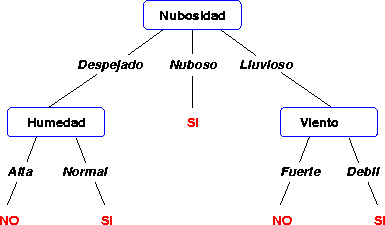
\includegraphics[scale=0.5]{img/tenis_decision_tree.png} }
			\caption[Árbol de decisión]{Árbol de decisión. Imagen extraida de Mitchell, T.M. (1997) \textit{Machine Learning}, McGraw-Hill.}
			\label{fig: Arbol de decision}
		\end{figure}
		
	Los algoritmos para entrenar un árbol de decisión usualmente trabajan de \textit{arriba hacia abajo}(\textit{top-down}, por su denominación en inglés) \cite{LROM05}. Dado un conjunto de características iniciales, en cada nodo del árbol, los algoritmos utilizan una función que evalúa cúal es el atributo más apropiado para representar al nodo y en base a eso dividen el conjunto inicial en dos o más partes. La elección de que función utilizar para realizar estas decisiones no es sencilla. En algunos casos, lo que se busca es generar un árbol de decisión óptimo que reduzca el error de generalización, en otros, se busca reducir el número de nodos o la profundida del árbol \cite{LROM10}. Este proceso continúa de manera recursiva hasta que el subconjunto de características en un nodo tiene el mismo valor para la variable objetivo, sea una clase o un valor numérico, o cuando las divisiones no agregan ningún valor a las predicciones. Este proceso es una estrategia muy común al momento de entrenar un árbol de decisión a partir de datos y es un ejemplo de \textit{algoritmo ambicioso}(\textit{greedy algorithm}, por su traducción al inglés). Si se considera nuevamente el ejemplo de la Figura \ref{fig: Arbol de decision}, se puede ver que los atributos, si bien son pocos, están bien ubicados en los nodos del árbol. En cambio, si se intercambian los nodos con los atributos \textit{humedad} y \textit{viento}, entonces el preguntar por la humedad sabiendo que el día está lluvioso no aporta información al momento de tomar una decisión.
	
	Cada algoritmo tiene su propio método al momento de dividir los nodos y decidir cuál es la mejor división que conlleve a disminuir los errores de clasificación. Por ejemplo, los algoritmos \textit{ID3 y C4.5}, \cite{QuinlanID3, QuinlanC45}, el primero precursor del segundo, utilizan el concepto de \textit{entropía} o \textit{entropía de información} para elegir al atributo que va a dividir el conjunto de características y que obviamente va a representar al nodo en el árbol. La entropía se la define como la medida de incertidumbre de una variable aleatoria.  Básicamente, dado un conjunto de características $S$, se itera sobre cada atributo no usado del mismo y se calcula la entropía sobre el mismo de la siguiente manera:
	\begin{align}
		\eta(S) = -\sum_i P(s_i)log_{2}P(s_i)
	\end{align}
	donde $S$ es nuestro conjunto conformado con los posibles valores $\{ s_1,\dots, s_n \}$ y $P( \cdot )$ es la función de probabilidad. Posteriormente, se elige aquel atributo que tenga menor entropía, mayor ganancia de información, y se lo utiliza para partir el conjunto $S$. Construir un árbol de decisión se basa en encontrar atributos que retornen la mayor ganancia de información con lo cual se obtienen ramas más homogéneas.
	
	Los árboles de decisión crecen hasta que se cumplen ciertos criterios: que se haya alcanzado la máxima profundidad del árbol, que todas las instancias del conjunto de entrenamiento pertenezcan a un solo valor de salida, entre otros \cite{LROM10}.

	Como expresan O. Maimon y L. Rokach en \cite{LROM10}, se puede dar el caso de que el árbol resultante sea excesivamente complejo, por ejemplo, al tener demasiados parámetros relativos al número de observaciones. Esto es lo que se conoce como \textit{sobreajuste} (\textit{overfitting}, de su traducción al inglés). Un modelo que ha sido sobreajustado, tendrá generalmente una baja tasa de predicción. Este tipo de problemas se generan cuando se eligen pobremente los criterios de parada. El caso contrario generaría árboles pequeños o débilmente ajustados. Los autores destacan que una forma de solucionar el sobreajuste es utilizando la técnica de \textit{poda} (\textit{pruning}, de su traducción al inglés). La poda reduce el tamaño de los árboles de decisión eliminando secciones del mismo que provean poca capacidad para clasificar instancias. El objetivo es tanto la reducción de la complejidad del clasificador como así también mejorar la performance a través de la reducción del sobreajuste.
	
	%La entropía, se la define como la medida de incertidumbre en una variable aleatoria y usualmente es medida en \textit{bits, nats o bans}. Para entender el concepto, consideremos el siguiente ejemplo: procedemos a tirar una moneda, si las probabilidades de que salga cara o cruz en la misma son iguales, es decir, la moneda es ``justa'' entonces decimos que la entropía es alta. Dicho de otra manera, no hay forma de predecir con anticipación cual va a ser el resultado. En cambio, si la moneda estuviese alterada y tuviese dos caras entonces la entropía es nula o cero lo cual nos quiere decir que la salida puede ser predecida perfectamente. Formalmente, se define la entropía $\eta$ de una variable aleatoria discreta $X$ con posibles valores $\{ x_1,\dots, x_n \}$ y función de probabilidad $P(X)$ de la siguiente manera:
	%\begin{align}
	%	\eta(X) = E[I(X)] = E[-ln(P(X))]
	%\end{align}
	%donde $E$ es el valor esperado e $I$ es el contenido de información de $X$ ($I(X)$ es en sí misma una variable aleatoria). Cuando se considera una muestra finita, podemos escribir:
	%\begin{align}
	%	\eta(X) = \sum_i P(x_i)I(x_i) = -\sum_i P(x_i)log_{b}P(x_i)
	%\end{align}
	%donde $b$ es la base del logaritmo usado (comúnmente se usa $2$, $10$ o el número de Euler $e$)

		
	%\subsubsection{Árbol aleatorio}

	Un árbol aleatorio o random tree, es un árbol construido al azar a
        partir de un conjunto de posibles árboles que tienen $K$
        características aleatorias en cada nodo. ``Al azar'' en este contexto
        significa que cada árbol tiene la misma chance de ser muestreado. Los
        árboles aleatorios pueden ser generados eficientemente y una
        combinación de conjuntos grandes de estos generalmente conlleva a
        modelos precisos.


        \JS{no queda claro de que se trata. Se puede desarrollar un poco mas}
		
	\subsubsection{Random Forest}

	\paragraph{Árbol aleatorio} ~\\
	
	Para comprender que es un árbol aleatorio, es necesario comprender que es un \textit{proceso estocástico}.
	
	Un proceso estocástico, es un proceso que se caracteriza por su indeterminación. Dicho de otra manera, la evolución de este, puede ir por muchos caminos posibles, incluso si conocemos el punto de partida (o condición inicial). Se diferencian de los procesos determinísticos, ya que estos últimos evolucionan de una sola manera, es decir, que no involucran la aleatoriedad en el desarrollo de los futuros estados del mismo.	
	
	Teniendo en cuenta este concepto luego, podemos decir, que un árbol aleatorio es un árbol construido a través de un proceso estocástico. Es decir, cada nodo del árbol se construye a partir de un proceso aleatorio que le asigna su valor. Dentro de los árboles aleatorios más comunes, podemos encontrarnos a  los \textit{árboles binarios} los cuales son construido insertando un nodo a la vez de acuerdo a una permutación aletoria.

	\paragraph{Random Forest} ~\\

	\textit{Random Forest} o \textit{bosque aleatorio} es un método de aprendizaje conjunto o\textit{ ensemble learning} para la clasificación o regresión. Es un clasificador que consiste en una colección de clasificadores con estructura de árbol $\{h(x,\Theta_k), k = 1,\dots\}$, donde $\{\Theta_k\}$ son vectores aleatorios independientes e identicamente distribuidos ($\Theta_k$ representa los parámetros para la construcción del $k$-esimo árbol) y $h(x,\Theta_k)$ es un clasificador donde $x$ es un vector de entrada. Luego, dada una entrada $x$, cada árbol emite un único voto para la elección de la clase más popular para $x$ \cite{Breiman01}.

	El algoritmo de entrenamiento para random forest aplica la técnica general de \textit{bootstrap aggregating}(agregación bootstrap) o \textit{bagging}(embolsado). Esta técnica fue desarrollada también por Breiman en 1996 ~\cite{LBreiman96} y es un método para generar múltiples versiones de un predictor y usar estos para obtener un predictor agregado. Para tener una idea más clara del concepto, consideremos el siguiente ejemplo basado en el trabajo de Breiman. Supongamos que tenemos $L = \{ (x_n,y_n), n = 1,\dots, N (N \in \mathbb{N}) \}$ el cual es un conjunto de aprendizaje donde $x_n$ son valores de entrada e $y_n$ son etiquetas de clase o valores numéricos. Supongamos también que tenemos una forma de generar un predictor de la forma $\varphi(x,L)$ a partir de $L$ tal que $ \varphi(x,L) = y $. Por último, supongamos que nos dan un conjunto de predictores $\{ L_k \}$ donde cada uno consiste en $N$ observaciones independiente bajo la misma distribución de $L$. El objetivo de Breiman en su trabajo, es que usando $\{ L_k \}$ se obtenga un predictor mejor que el establecido anteriormente $\varphi(x,L)$. La única restricción, es que se nos obliga a trabajar solamente con el conjunto de predictores $\{ \varphi(x, L_k)\} $.

	Para resolver este problema, Breiman estableció el siguiente criterio. Si la respuesta $y$ era un valor numérico luego, se reemplaza a $\varphi(x,L)$ por el promedio del conjunto de predicotres $ \{ \varphi(x, L_k) \} $ sobre $k$. Es decir, $\varphi_A(x) = E_L\varphi(x,L)$ donde $E_L$ denota la esperanza sobre $L$, y el subíndice $A$ en $\varphi_A$ denota la agregación. En cambio, si $\varphi(x,L)$ predecía una etiqueta de clase $j \in \{ 1,\dots, J \} $, luego un método para agregar todos los predictores era a través del voto. Es decir, para el autor $N_j = \{ k;\varphi(x, L_k) = j \}$ y se toma a $\varphi_A(x) = argmax N_j$.

	El problema principal, es que generalmente se tiene sólo un conjunto de aprendizaje $L$. Para esto, Breiman considera que se puede imitar el procedimiento anterior tomando repetidas muestras bootstrap $\{ L^{B} \}$ a partir de $L$, y formar $\{ \varphi(x, L^{B}) \}$. Si $y$ es numérica luego, toma $\varphi_B$ como
	\begin{align*}
		\varphi_B(x) = av_B\varphi(x,L^{B}).
	\end{align*}

	Si $y$ es una etiqueta de clase, luego el conjunto  $\{ \varphi(x, L^{B}) \}$ vota para formar $\varphi_B(x)$. El autor a este procedimiento lo llama  \textit{bootstrap aggregating} o \textit{bagging}.

	Cabe aclarar, que cada $L_i \in \{ L^{B} \}$ consta de $N$ muestras obtenidas al azar, pero con reemplazo, de $L$. Cada $(x_n, y_n)$ puede aparecer repetido una cierta cantidad de veces o no en $L_i$.

	Se puede aplicar \textit{bagging} para generar un algoritmo para árboles de decisión o regresión. Dado un conjunto de aprendizaje $L$ como el explicado anteriormente, la técnica de bagging selecciona repetidamente muestras de bootstrap del conjunto de aprendizaje $L$ y ajusta los árboles a estas muestras:

	Para $b=1$ hasta $B$:
	\begin{itemize}
		\item Se realiza un muestreo, con reemplazo, de $n$ ejemplos de entrenamiento a partir de $L$; llamemos a esta muestra $L_b$.
		\item Entrena un árbol de decisión o regresión $f_b$ a partir de $L_b$.
	\end{itemize}

	Después del entrenamiento, las predicciones para ejemplos no vistos $x'$ se pueden realizar promediando las predicciones de todos los árboles de regresión en $x'$:
	$$\bar{f} = \frac{1}{B}\sum_{b=1}^B\bar{f_b}(x')$$
	o tomar el voto mayoritario en caso de árboles de decisión.

	En el algoritmo de arriba, B es un parámetro libre que indica la cantidad de árboles predictores que se van a emplear. Típicamente, algunos cientos o miles de árboles son usados, dependiendo del tamaño y naturaleza del conjunto de entrenamiento.

	El procedimiento anterior describe el algoritmo original de \textit{bagging} para árboles. Desafortunadamente, volver a correr el mismo algoritmo de aprendizaje en diferentes subconjuntos de los datos puede resultar en predictores altamente correlacionados, lo cual limita la reducción de varianza. La técnica conocida como \textit{random forest}, construye árboles basados en un subconjunto de variables de entrada elegidas al azar.

	Cada árbol es construido siguiendo el siguiente algoritmo:
	\begin{itemize}
		\item Si el número de muestras en el conjunto de entrenamiento es $N$, muestrear $N$ casos aleatoriamente - pero con reemplazo, a partir de los datos originales. Esta muestra va a ser el conjunto de entrenamiento para la construcción del árbol.
		\item Si hay $M$ variables de entrada, se especifica un número $m<<M$ (constante durante el crecimiento del bosque o forest) tal que en cada nodo se seleccionen $m$ variables al azar de las $M$. Posteriormente se eligen entre las $m$ variables aquellas que mejor dividan al nodo, es decir, aquellas que generen al final un árbol compacto y simple.
		\item Cada árbol se construye hasta su máxima extensión posible. No hay pruning(poda).
	\end{itemize}
	Las ventajas random forests son:
	\begin{itemize}
		\item Correr eficientemente en grandes bases de datos.
		\item Poder manejar cientos de variables entrantes sin excluir ninguna.
		\item Dar estimaciones de qué variables son importantes en la clasificación.
		\item Ofrecer un método experimental para detectar las interacciones de las variables.
	\end{itemize}
	Las desventajas de este algoritmo se pueden resumir en estos puntos:
	\begin{itemize}
		\item A diferencia de los árboles de decisión, la clasificación hecha por random forests es difícil de interpretar por el hombre.
		\item Si los datos contienen grupos de atributos correlacionados de relevancia similar para el rendimiento, entonces los grupos más pequeños están favorecidos por sobre los grupos más grandes.
	\end{itemize}
	

	
	\subsubsection{Random Ferns} 
\label{subsection:ferns}
	
		Random Ferns es un clasificador propuesto por Ozuysal et. al.~\cite{Ozuysal}. Al igual que Random Forest, es un clasificador multi-clase, compuesto de un determinado número de entidades o clasificadores y es una alternativa más rápida y simple que este último. En oposición a Random Forest, Ferns es una estrutura no jerárquica donde cada entidad que constituye el clasificador es básicamente un conjunto de prueba binario. En Random Forest el conjunto de prueba de cada árbol es la colección de diferentes pruebas que se distribuyen a lo largo de los nodos que forman el árbol. Debido a la estructura plana de cada entidad en un clasificador Ferns, el conjunto de prueba es una sencilla lista ordenada de las posiciones de los features o características a ser evaluados.
		
		Sea $c_i, i=1,\dots,H$ el conjunto de clases y  sea $f_j, j=1,\dots,N$ el conjunto de características binarias. Formalmente, se busca:
		$$\underset{c_i}{argmax}P(C=c_i \vert f_1,f_2,\dots,f_N),$$
		donde $C$ es una variable aleatoria que representa a la clase. La fórmula de Bayes produce:
		$$P(C=c_i \vert f_1,f_2,\dots,f_N) = \frac{P(f_1,f_2,\dots,f_N \vert C=c_i)P(C=c_i)}{P(f_1,f_2,\dots,f_N)}$$
		Asumiendo una probabilidad uniforme a prior $P(C)$, dado que el denominador es simplemente un factor de escala que es independiente de la clase, el problema se reduce a encontrar:
		\begin{align}\label{eq:class}
			c_i  = \underset{c_i}{argmax}P(f_1,f_2,\dots,f_N \vert C=c_i)
		\end{align}
		Por lo tanto, una completa representación de la probabilidad conjunta en la ecuación \ref{eq:class} no es factible dado que requeriría estimar y almacenar $2^N$ entradas por cada clase. Una forma de comprimir la representación es asumir independencia entre características. Una versión extrema es la de asumir independencia completa, es decir
		$$P(f_1,f_2,\dots,f_N \vert C=c_i) = \prod_{j=1}^NP(f_j \vert C=c_i)$$
		Sin embargo, esto ignora completamente la correlación entra las características. Para hacer el problema manejable, un buen método es partir las características en $M$ grupos de tamaño $S=\lfloor \frac{N}{M} \rfloor$. Estos grupos son los que se denominan \textit{ferns} y se calcula la probabilidad conjunta de cada característica en cada fern. La probabilidad condicional se vuelve
		\begin{align}\label{eq:class2}
			P(f_1,f_2,\dots,f_N \vert C=c_i) = \prod_{k=1}^MP(F_k \vert C=c_i)
		\end{align}
		donde $F_k = \{ f_{\sigma(k,1)},f_{\sigma(k,2)},\dots,f_{\sigma(k,S)}, k=1,\dots,M \}$ representa el $k^{th}$ fern y $\sigma(k,j)$ es una función de permutación aleatoria con rango $1,\dots,N$. De ahí que se sigue un enfoque bayesiano Semi-Na\"{i}ve modelando algunas de las dependencias entre características.

		La fase de entrenamiento estima la probabilidad condicional de clase $P(F_m|C=c_i)$ para cada fern $F_m$	 y cada clase $c_i$, como está descripto en la ecuación \ref{eq:class2}. Para cada fern $F_m$ escribimos estos términos como:
		\begin{align}
			p_{k,c_i} = P(F_m = k | C = c_i)
		\end{align}
		donde se simplifica la notación considerando que $F_m$ es igual a $k$ si el número en base $2$ formado por los features binarios de $F_m$ tomados en secuencia es igual a $k$. Con esta convención, cada ``fern'' puede tomar $K=2^S$ valores, y para cada uno, es necesario estimar $p_{k,c_i}, k=1,2,\dots,K$ bajo la restricción
		\begin{align*}
			\sum_{k=1}^Kp_{k,c_i} = 1
		\end{align*}		
		
		El enfoque más simple sería asignar la estimación de máxima verosimilitud a estos parámetros a partir de las muestras de entrenamiento. Para el parámetro $p_{k,c_i}$ es
		\begin{align*}
			p_{k,c_i} = \frac{N_{k,c_i}}{N_{c_i}}
		\end{align*}
		donde $N_{k,c_i}$ es el número de muestras de entrenamiento de la clase $c_i$ y $N_{c_i}$ es el número total de muestras para la clase $c_i$. Estos parámetros por lo tanto, pueden ser estimados para cada fern independientemente.
		
		En la práctica sin embargo, este simple esquema da pobres resultados porque si ninguna muestra de entrenamiento para la clase $c_i$ evalua a $k$, lo cual puede pasar con facilidad cuando el número de muestras no es infinitamente largo, ambos $N_{k,c_i}$ y $p_{k,c_i}$ serán cero. Dado que se multiplica $p_{k,c_j}$ por todos los ferns, esto implica que, si el fern evalua a $k$, la correspondiente muestra nunca va a ser asociada a la clase $c_i$, sin importar la respuestas de los otros ferns. Para superar este problema, se considera $p_{k,c_i}$ de la siguiente manera
		\begin{align}
			\label{eq:Laplace-Smoothing}
			p_{k,c_i} = \frac{N_{k,c_i} + N_r}{N_{c_i} + K \times N_r},
		\end{align}
		donde $N_r$ representa un término de regularización. La ecuación \ref{eq:Laplace-Smoothing} usa la técnica de \textit{suavizado de Laplace} (\textit{Laplace smoothing}, por su traducción al inglés) que es usada en estadística para suavizar datos categóricos. Si una muestra con un valor específico de fern no se encuentra durante el entrenamiento, este esquema, aún le va a asignar un valor distinto de cero a la probabilidad correspondiente.
	
	\newpage
\subsection{Clasificación de imágenes naturales}

	\subsubsection{Características}

Las características en las imágenes naturales son muy variadas. Dentro de las mismas podemos encontrar las variaciones de intensidad en la iluminación, la resolución, el ángulo en el que son tomadas, el fondo, las texturas, entre otros. Mas específicamente, dependiendo del objeto que se esté analizando, por ejemplo, texto, surgen más características como el tipo de fuente, el tamaño, la posición y orientación de los caracteres, la contaminación que pueda llegar a tener el texto por suciedad u oclusión, etc. La infita variedad que es posible encontrar en este tipo de imágenes, dificultan el trabajo de reconocimiento sobre ellas por lo que, en general, es necesario realizar un pre-procesamiento antes de usarlas.

	En el caso del reconocimiento de texto, dada la gran cantidad de formas en que se puede encontrar la imagen de un carácter, es necesario encontrar algún método que extraiga las características mas representativas para poder distinguilo. Para poder analizar los caracteres en las imágenes naturales, uno de los enfoques que adoptan Wang et al. en \cite{wang} es el de trabajar con el descriptor HOG de cada imagen. Para poder entender que es un descriptor HOG (que se detalla en \ref{subsection:hog}), primero es necesario comprender el concepto de gradiente que se explica a continuación.
	
	%\input{capitulo2/natural_imgs.tex}
	
\subsubsection{Gradientes}
\label{subsubsection: Gradientes}

Sea $f(x_1,\dots,x_n)$ una función escalar de múltiples variables. Como expresa Gonzales et. al. en \cite{GonWoods}, el gradiente de $f$ es un vector que apunta en la dirección donde se registra la mayor tasa de incremento de la función. Su magnitud es la pendiente del gráfico en esa dirección. Es la generalización del concepto de derivada en funciones de múltiples variables.
		
	El gradiente de la función $f$ descrita anteriormente, es denotado como $\nabla f$ donde $\nabla$ (el símbolo nabla) denota el operador diferencial. El gradiente de $f$ es definido como el único campo vectorial cuyo producto punto con cualquier vector $v$ en cada punto $x$ es la derivada direccional de $f$ a lo largo de $v$. Es decir,
		 \begin{align*}
		 	(\nabla f(x))\cdot v = D_v f(x)
		 \end{align*}
		 
	En un sistema de coordenadas rectangular, el gradiente es el campo vectorial cuyos componentes son las derivadas parciales de $f$:
		 
		 \begin{align*}
		 	\nabla f(x) = \frac{\partial f}{\partial x_1}\mathbf{e}_1 + \cdots + \frac{\partial f}{\partial x_n }\mathbf{e}_n
		 \end{align*}
	donde los $\mathbf{e}_i$ son vectores unitarios ortogonales que apuntan en la dirección de coordenadas.

	En el procesamiento de imágenes, un gradiente es un cambio direccional en la intensidad o color de la imagen. En \cite{DJacobs}, Jacobs explica que el vector gradiente se forma combinando la derivada parcial de la imagen en las direcciones $x$ e $y$. Se puede expresar del a siguiente forma:
		\begin{align}
			\nabla I = \left( \frac{\partial I}{\partial x} , \frac{\partial I}{\partial y} \right)
		\end{align}	
		
	donde \textit{I}: $\mathbb{R}^{2} \rightarrow [0, 1]$ es la ``función intensidad'' que asigna un valor de intensidad a cada pixel (par (x,y)) de la imagen. Según Jacobs, cuando determinamos la derivada parcial de $I$ respecto de $x$, determinamos la rapidez con que la imagen cambia de intensidad a medida que $x$ cambia. Para funciones continuas, $I(x,y)$, podemos expresarlo de la siguiente manera:
	\begin{align}
		\frac{\partial I(x,y)}{\partial x} = \lim_{\nabla x\rightarrow 0} \frac{I(x + \nabla x, y) - I(x,y)}{\nabla x}	
	\end{align}
	
	 El cálculo de los gradientes de una imagen es útil ya que sirve, por ejemplo, para realizar detección de bordes de un objeto. La detección de bordes busca identificar puntos en una imagen en donde el brillo de la misma cambie de manera abrupta o, más formalmente, tenga discontinuidades. El propósito de esto es capturar eventos importantes o cambios en las propiedades de una imagen. En este caso, después de que los gradientes han sido computados, los píxeles con alto valor de gradiente son elegido como posibles bordes. Los píxeles con el valor de gradiente más alto en la dirección del gradiente se convierten en píxeles de borde. Los gradientes, también pueden ser usados en aplicaciones que realizan reconocimiento de objetos o correspondencia de texturas.	 
	
	\subsubsection{Características locales}

		\input{capitulo2/sift.tex}	
	
		\input{capitulo2/hog.tex}
	
	\subsubsection{Reconocimiento de objetos}



	\newpage	
\section{End-to-end scene text recognition}
	
	\subsection{Introducción}

	En el trabajo que realizaron Wang et al., los autores identificador el problema que había al detectar y reconocer palabras en imágenes naturales. Ellos identifican, que si bien las actuales aplicaciones de OCR se manejan bien con documentos escaneados, todavía encuentran problemas cuando tratan de procesar texto adquirido en entornos naturales (también referido como texto de escena). Este tipo de texto se ha vuelto más frecuente debido al aumento de dispositivos que son capaces de extraer dicha información, sean estos celulares, tabletas o cámaras.
	
	Durante la competencia de ICDAR (\textit{International Conference on Document Analysis and Recognition}) en 2003, los organizadores tenían como objetivo ver cual era el estado del arte en las diferentes etapas del reconocimiento de texto en escenas naturales. Observaron que habían imágenes con texto que los motores de OCR del momento no podían procesar, por lo tanto, decidieron dividir el problema general que era reconocer palabras en escenas naturales en tres subproblemas:
	
	\begin{itemize}
		\item \textbf{La clasificación de caracteres recortados.}
		
		En este problema se consideran imagenes de caracteres extraidas de escenas naturales. Las imagenes contienen exclusivamente un sólo carácter y sus tamaños se ajustan a las dimensiones del caracter tal como se puede apreciar en la Figura \ref{fig: Caracteres recortados}. El objetivo es identificar qué carácter está reflejado en la imagen a partir de un conjunto predefinido de caracteres que hacen al problema.

		Una de las dificultades de este problema es que algunos caracteres son muy difíciles de dicernir entre sí, por ejemplo, si consideramos las letras mayúsculas y las minúsculas por separado, luego una ``Z'' es muy difícil de dicernir de una ``z''. Incluso se puede dar lugar a la confusión entre distintos símbolos, por ejemplo, la ``O'' (letra o mayúscula) y el número ``0'' o el número ``6'' y la ``G'' (letra ``g'' mayúscula).
						
		Otro elemento que se tiene que tener presente al momento de clasificar caracteres, es el tipo de características locales que se van a obtener de cada imagen. Como se ha explicado en la sección \ref{subsection:feature}, las características son importantes dado que representa los aspectos o cualidades más significativas de un objeto. Si se hace una buena elección de las características locales, se va a ver reflejado en la performance de clasificación.
		
		Las condiciones en que fueron tomadas las imágenes donde se extrajeron los caracteres influye posteriormente en su reconocimiento. Por ejemplo, las variaciones en las condiciones de iluminación, oclusión, posicionamiento al momento de tomar la imagen, etc. Para resolver esto, se puede realizar un pre-procesamiento que ayude a ``limpiar'' la imagen para poder facilitar su reconocimiento posterior.
		
	\begin{figure}[htbp]
		\centering
  		\centerline{ 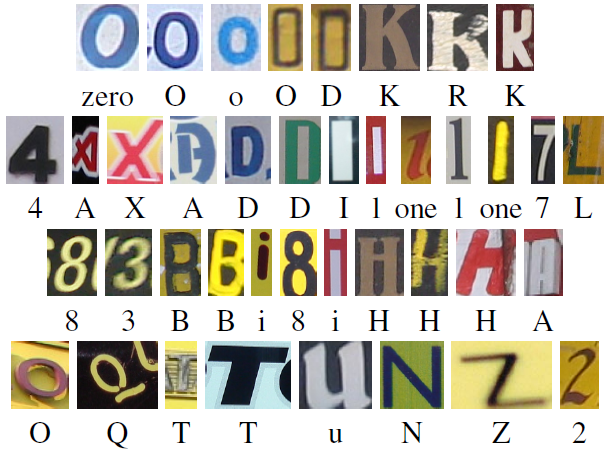
\includegraphics[scale=0.5]{img/hog/confusing_english.png} }
		\caption[Clasificación de caracteres recortados]{Conjunto de caracteres recortados. Imagen extraida del paper de T. E. de Campos et. al. \cite{dCBV09}}
		\label{fig: Caracteres recortados}
	\end{figure}
		
		\item \textbf{Detección de zonas con texto en la imagen.}
		
		Este problema involucra la detección de zonas de la imagen que pueden contener texto. Esto se realiza con el objetivo de priorizar estas regiones en procesamientos posteriores para reducir la complejidad del problema del análisis de texto. La figura \ref{fig: Zona texto} expone un ejemplo de este problema.
		
		Para poder resolver este problema, se debe considerar que las palabras que conforman el texto a detectar, pueden haber sido adquiridas a distintas escalas. Tal es el caso del texto de casi la mayoría de los carteles publicitarios que es posible encontrar en las calles de una ciudad. Otro factor a considerar es la inclinación del texto que puede darse por la posición del observador. Además, esta tarea se dificulta si consideramos, al igual que en el reconocimiento de caracteres, las condiciones de la imagen (iluminación, distorsiones, estilo y fuente de las palabras en el texto, etc).
		
		En el trabajo de Chen H. et. al. \cite{ChenH11}, los autores destacan que hay dos categorías al momento de diferenciar las técnicas de reconocimiento de texto. La primera categoría, son las técnicas \textit{basadas en textura} (\textit{texture based} de su traducción al inglés) que destacan al texto como una ``textura'' especial que es distinguible del fondo. Las características se extraen de ciertas regiones de la imagen y se utiliza un clasificador para identificar la existencia de texto. La segunda categoría, son las técnicas basadas en \textit{componentes conectados} (\textit{connected component} de su traducción al inglés), donde se extraen regiones de la imagen y se utilizan restricciones geométricas para descartar candidatos que no sean texto.
		
	\begin{figure}[htbp]
		\centering
		\centerline{ 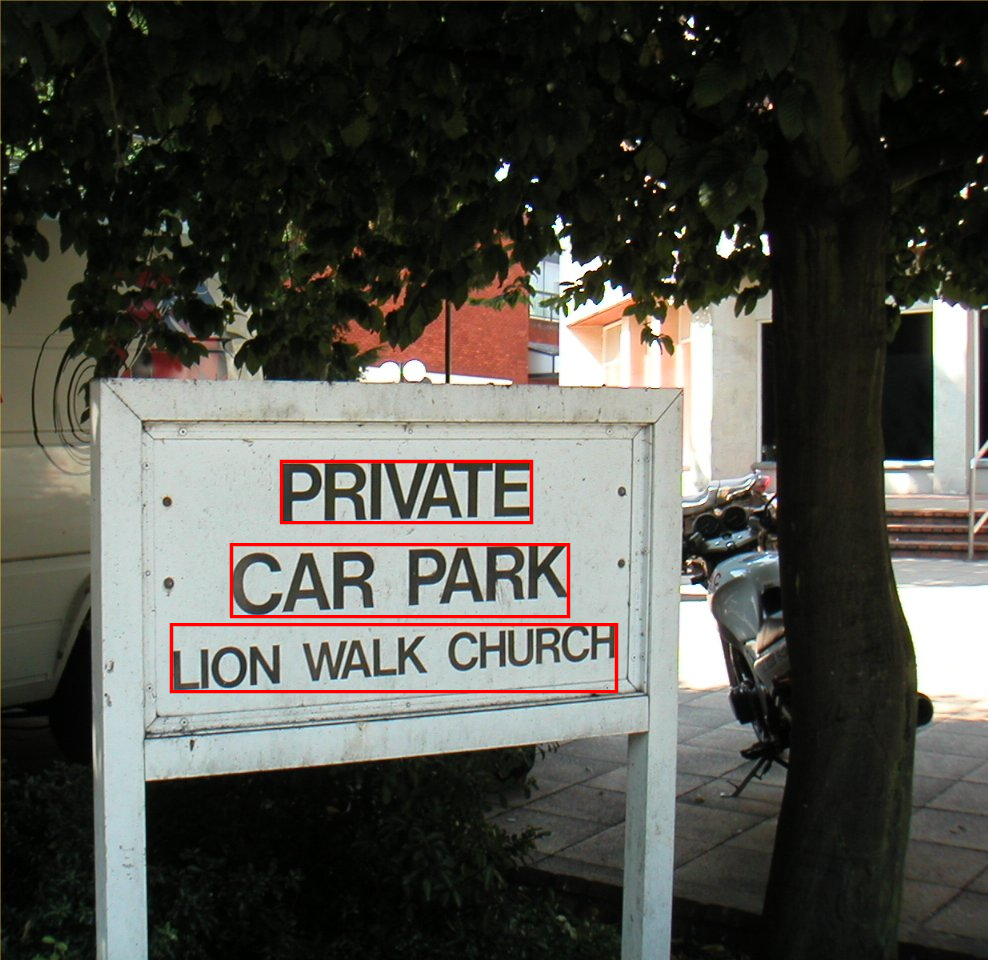
\includegraphics[scale=0.20]{img/zone_with_text.png} }
		\caption[Detección de zonas con texto]{Imagen natural donde las zonas con texto están encasilladas.Imagen tomada del sitio \url{http://libccv.org/post/introducing-ccv-milestone/} }
		\label{fig: Zona texto}
	\end{figure} 
		
		\item \textbf{El reconocimiento de palabras recortadas.}

		En este problema se busca identificar las palabras que se encuentran dentro de las imágenes recortadas. Al igual que el problema del reconocimiento de caracteres, en este problema, cada imagen contiene una sola palabra y la dimensiones de estas imágenes se ajustan a las palabras tal como se puede ver en la Figura \ref{fig: Reconocimiento palabras}.
		
		Una de las dificultades surgen en este problema al manipular imágenes naturales, son las condiciones en que estas fueron adquiridas. Como se explicó anteriormente, las variaciones en la iluminación, la oclusión, entre otros, generan problemas en el reconocimiento. 

		Uno de los métodos que se utiliza en la actualidad y se considera estado del arte son las estructuras pictóricas. Este método fue usado por Wang y Belongie en \cite{WB10}, donde en base a un lexicón (conjunto de palabras), miden la configuración de cada carácter de cada palabra en la imagen. Básicamente toma la ubicación y el puntaje de los caracteres detectados como entrada y encuentra la configuración óptima para una palabra en particular \cite{wang}. Una de las particularidades de este trabajo, es que requiere de un clasificador de caracteres para poder posteriormente realizar el reconocimiento de palabras.
	
	\begin{figure}[htbp]
		\centering
		\centerline{ 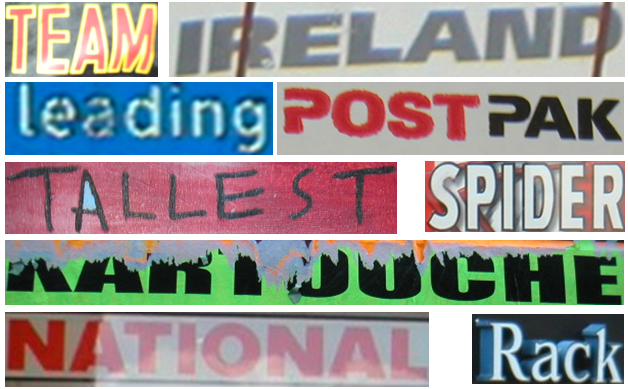
\includegraphics[scale=0.30]{img/cropped_words.png} }
		\caption[Reconocimiento de palabras recortadas]{Conjunto de palabras recortadas de diferentes escenas naturales. Imagen extraida del sitio de \textit{Graphics and Media Lab}, \url{http://graphics.cs.msu.ru/en/science/research/machinelearning/text}}
		\label{fig: Reconocimiento palabras}
	\end{figure}
		
	\end{itemize}

	Dada esta problemática, Wang et al. se enfocaron en un caso especial del reconocimiento de texto de escena donde tenían a disposición un listado de palabras (i.e, un lexicón) para detectar y leer.
		
	Para esto, ellos construyen y evalúan dos sistemas. En el primero, evalúan la performance en la detección y el reconocimiento de palabras de un enfoque con dos etapas que consiste en un detector de texto considerado estado del arte y un destacado motor de OCR. El segundo, es un sistema arraigado en el reconocimiento de objetos genéricos, el cual es una extensión de un trabajo que realizaron anteriormente \cite{WB10}. En \cite{WB10}, los autores consideran a las palabras como categorías de objectos en sí mismas y realizan reconocimiento sobre las categorías de las palabras. Utilizan técnicas propias del reconocimiento de categorías genéricas y las aplican al reconocimiento de palabras. Asi como podemos tener muchas imágenes que representen el objeto ``vehículo'', también es posible aplicar la misma idea para la palabra ``door'' como muestra la Figura \ref{fig: Reconocimiento generico}. La figura representa una analogía al reconocimiento de objetos genéricos.
	
	En \cite{wang}, los autores remarcan que para poder lograr el reconocimiento de palabras en imágenes, es necesario en primera instancia tener un clasificador de caracteres. Este trabajo se enfoca en el reconocimiento de caracteres en ventanas, es decir, imagenes de caracteres recortados de escenas naturales. 
	
	
	
	\begin{figure}[htbp]
		\centering
		\centerline{ 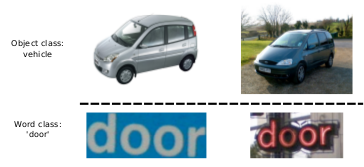
\includegraphics[scale=0.7]{img/object_recognition.png} }
		\caption[Reconocimiento generico de objetos]{Reconocimiento de palabras. Se considera a la palabra como una categoría de objeto al igual que la categoría ``vehiculo'' presentada en la parte superior de la imagen.}
		\label{fig: Reconocimiento generico}
	\end{figure}
	
	
	\subsection{Reconocimiento de caracteres}

	\begin{itemize}
		\item Algoritmos usados
			\begin{itemize}
				\item Introducción a Random Ferns: explicar el algoritmo y porqué lo usaron.
				\item HOG: hacer una ligera mensión de su uso. Los detalles van a estar en la sección correspondiente en el capítulo 2.
				\item non-maximal suppression (NMS) \JS{esto
                                    está asociado a esquemas de detección del tipo
                                    ``sliding window''}
			\end{itemize}
		\item Datasets usados \JS{no pondría nada sobre datasets acá,
                    sino mas bien una discusión sobre la necesidad de usar
                    datasets grandes para cubrir la variabilidad de apariencias
                  que aparecen en img reales}
			\begin{itemize}
				\item Aca puede ir una explicación del uso de datos sintéticos.
			\end{itemize}
	\end{itemize}
	
	\subsection{Reconocimiento de palabras}
	\begin{itemize}
		\item Introducción a Pictorial Structures (Teoría)
		\item Uso de PS + Lexicón
		\begin{itemize}
			\item Algoritmo PLEX
		\end{itemize}
		\item Re-scoring y NMS
		\begin{itemize}
			\item Problemas con PLEX
		\end{itemize}
		\item Implementación
	\end{itemize}
	
	Para detectar palabras en una imagen, uno de los métodos que usan Wang et al., son las \textit{estructuras pictóricas} (\textit{pictorial structures}, de su traducción al inglés). Este enfoque toma las ubicaciones y puntajes de los caracteres detectados como entrada y encuentra la configuración óptima de una palabra específica. Formalmente, dada una palabra $w=(c_1,\dots , c_n)$ de $n$ caracteres de un lexicó, sea $L_i$ el conjunto de ubicaciones detectadas para el $i$-esimo carácter de $w$, y $u(l_i, c_i)$ sea puntuación de una detección particular en la ubicación $l_i \in L_i$ (obtenida a través del clasificador Random Ferns). La idea de este método, como ya se dijo, es obtener una configuración óptica $L^{*}=(l_1^{*}, \dots, l_n{*})$ optimizando la siguiente función:
	\begin{align}
		L^{*} = \underset{\forall i, l_i\in L_i}{argmin}\left( \sum_{i=1}^n -u(l_i, c_i) + \sum_{i=1}^{n-1} d(l_i,l_{i+1}) \right)
	\end{align}		
	
	donde $d(l_i, l_j)$ es el costo asociado de incorporar disposición espacial y similitud de escala entre dos caracteres vecinos. Usando programación dinámica se puede optimizar la ecuación anterior. Sea $D(l_i)$ el costo de colocación óptima de los caracteres $i+1$ a $n$ con la ubicación del $i$-esimo carácter fijado en $l_i$:
	\begin{align}
		D(l_i) = -u(l_i,c_i) + \underset{l_{i+1}\in L_{i+1}}{min} d(l_i,l_{i+1}) + D(l_{i+1})
	\end{align}
	Dada la naturaleza recursiva de $D(\cdot)$ se puede encontrar la configuración óptima pre-computando $D(l_n) = -u(l_n,c_n)$ para cada $l_n \in L_n$ y posteriormente trabajando para atrás hacia la primera letra.
	
	Una forma de extender dicha configuración para obtener las configuraciones de múltiples palabras, consiste en el uso de un algoritmo desarrollado por los autores denominado \textit{PLEX}. Consideremos el siguiente ejemplo, extraido del trabajo de Wang et al., el cual refleja muy bien el procedimiento. Supongamos que tenemos dos palabras en nuestro lexicón $\{$``ICCV'', ``ECCV'' $\}$. El valor de $D(l_2)$ es el mismo pues ambas palabras comparte el mismo sufijo ``CCV'', y por lo tanto puede ser computado una sola vez y usado para ambas palabras. Con esta idea en mente, se construye un árbol a partir de un lexicón donde cada letra de cada palabra del lexicón conforma un nodo y, empezando desde la última letra de la palabra, cada letra subsiguiente se encuentra en nivel inferior del árbol hasta alcanzar la primera letra (representada por un nodo coloreado o marcado como el inicio de la palabra). Con este enfoque, aquellas palabras que compartan un mismo sufijo, van a compartir el mismo recorrido en el árbol hasta que se separan. Cabe aclarar que el nodo raiz se lo considera ``vacio'' por lo cual la última letra de cada palabra representa el primer nodo descendiente de la raiz. En el peor de los casos, cuando dos palabras en un lexicón no comparte un sufijo común, este método es equivalete a realizar la configuración de cada palabra por separado.
	
	Unos de los problemas que presenta \textit{PLEX}, es que los puntajes no son compatibles para palabras de diferente longitud. El problema más imporante sin embargo, es que la función objetivo de las estructuras pictóricas captura solamente relaciones de a pares e ignora las características globales de la configuración.
	
	Dado esto, la última etapa del pipeline es realizar \textit{non-maximal suppression} sobre todas las palabras detectadas, Esto con el objetivo de incorporar algo de información global en esta última parte. Para eso, se vuelve a puntuar cada palabra retornada por \textit{PLEX} utilizando un clasificador \textit{Support Vector Machine} (\textit{SVM} por sus siglas en inglés).

	\RC{Falta experimentos}	
	


	\newpage
\section{Experimentos}

	\subsection{Diseño de los experimentos}

	\begin{itemize}
		\item Aca debería ir una descripción de los parámetros a usar en los experimentos con una explicación de lo que se espera obtener.
		\begin{itemize}
			\item Explicar para qué sirve cada parámetro
			\item Explicar los valores que se van a usar para cada parámetro
		\end{itemize}
	\end{itemize}

	Dada la gran cantidad de parámetros que hay en el sistema, la cantidad de experimentos para encontrar la mejor configuración es extensa.

        \paragraph{Generación de datos sintéticos}

	El primer parámetro a considerar es el tipo de conjunto de entrenamiento a evaluar, como se procederá a explicar en la próxima sección, tenemos un total de 20 conjuntos diferentes. Esto con el objetivo de evaluar la performance del clasificador en diferentes ámbitos. Los parámetros utilizados durante la creación de las imágenes sintéticas son, como se explicó en el capítulo anterior, escala, rotación, blur, ruido gaussiano e inclinación. Dado que hay un abanico bastante grande valores para asignarles a estas transformaciones, se decidió por asignarle a cada una un rango de valores los cuales si bien modificaban la imagen, no la hacían ilegible. Dado que los autores en \cite{wang} no especifican el rango de valores para las transformaciones afines que utilizan, se procedió a establecer el siguiente conjunto de rangos para todas las tranformaciones utilizadas:
	
	\begin{itemize}
		\item Inclinación: factor de inclinación $n \in [-0.20 ; 0.20]$
		\item Suavizado gaussiano (blur): $\sigma \in [0 ; 2]$
		\item Escala: es igual en ambos ejes $x=y \in [0.8; 1.25]$
		\item Rotación: en radianes $\theta \in (-0.1; 0.1)$
		\item Ruido gaussiano: $\sigma \in [1; 30]$
	\end{itemize}
	
	El hecho de no contar con una replica exacta del conjunto de datos sintéticos usados por Wang et al., los conjuntos generados con estos valores claramente van a ser distintos a los originales y por ende la comparación de resultados  en \ref{subsection:resultados} va a estar influida por la forma en que se generaron los conjuntos.
	
	\paragraph{Extracción de características con HOG}

	Posteriormente tenemos los parámetros propios que utiliza HOG para extraer las características de cada imagen. HOG hace uso de dos parámetros, la cantidad de \textit{orientaciones} y la cantidad de \textit{celdas por bloque}. Como se explicó en el capítulo anterior \ref{subsection:hog}, dada una imagen, esta se dividía en regiones llamadas celdas. Dentro de cada una se realiza el calculo de las orientaciones y posteriormente dado un bloque de celdas se extraía un histograma de orientaciones de todas las celdas involucradas. Dada la gran cantidad de combinaciones entre ambos parámetros, se decidió por utilizar los siguientes valores:
	
	\begin{itemize}
		\item Orientaciones: $\{8; 9\}$
		\item Celdas por bloque: $\{4; 9\}$
	\end{itemize}
	
	La elección de estos números se debe a que reducen la tasa de errores de clasificación. Un análisis similar se puede encontrar en \cite{DT05} donde los autores (quienes crearon HOG) analizan la mejor configuración para resolver el problema de detección de personas. Si bien el problema que se busca resolver en este trabajo es totalmente diferente, los parámetros que ellos usan para HOG muestran buenos resultados en este problema también.

	\paragraph{Binarización}

	HOG devuelve descriptores de tamaño fijo dependiendo de la cantidad de orientaciones y celdas por bloque que le asignemos. Lo que buscamos con establecer una longitud variable, es evaluar la perdida o ganancia de información sobre la imagen al realizar esto y ver si hay algun impacto en la performance al final. Para poder realizar este ``estiramiento'' o ``reducción'' de los vectores, nos aprovechamos del proceso de binarización explicado anteriormente. El impacto producido al realizar esto es notable y se va a detallar al final del capítulo. Las dimensiones con las que se trabajan es otro parámetro (para los experimentos con imágenes sintéticas y mixtas). Los valores con los que trabajamos son los siguientes:

	\begin{itemize}
		\item Dimensión del vector final: $\{ 240; 480; 1080; 2040;  4080 \}$
	\end{itemize}
	
	La elección de estas dimensiones está directamente relacionada con el siguiente parámetro que es la cantidad de \textit{grupos} por vector, por lo cual estas dimensiones tienen que ser divisibles por cada uno de los grupos a evaluar
	
	Como último parámetro a destacar en la binarización, y lo consideramos como uno de los más importantes, es el método aplicado al momento de generar el umbral de binarización. Como se podrá ver en la subsección de Resultados del capítulo 4, es muy grande el impacto obtenido en la precisión final del clasificador debido a este parámetro. La elección de qué método utilizar fue libre con el objetivo de evaluar cual era el que otorgaba mejores resultados. Se trabajaron con los siguientes métodos:

	\begin{itemize}
		\item Media
		\item Mediana
		\item Bootstrap
		\item Exponencial
	\end{itemize}
	
	Dado que los autores en \cite{wang} no especifican que método usaron al momento de binarizar los vectores. Proponemos estos cuatro métodos. Al igual pasó con los parámetros para generar los datos sintéticos, en el \cite{wang} no se aclara que método se utilizó para la binarización de los vectores, con lo cual todos los resultados obtenidos en los experimentos realizados con imágenes reales y sintéticas van a ser distintos de los originales por más de que, en el caso de las imágenes reales, se usen los mismos conjuntos de entrenamiento y prueba. \RC{Discutir esto, IMPORTANTE.}
		
	\paragraph{Entrenamiento}

	En la etapa de entrenamiento, hay 2 parámetros: la cantidad de bits por \textit{grupo} que determina finalmente la cantidad de grupos en la que se divide cada vector y \textit{alpha} que es un parámetro de inicialización para las tablas. La cantidad de grupos en las que se divide un vector impacta en el tamaño de las tablas y en la clasificación posterior. La cantidad bits denotan la cantidad de dimensiones de cada grupo, por lo cual  la cantidad de grupos esta dado por la división entre la dimensión total del vector y la dimensión del grupo.

	El parámetro \textit{alpha} es necesario ya que las tablas no se pueden inicializar con el valor $0$. Esto es debido ya que, como se explico en la sección \ref{subsection:ferns}, al momento de evaluar una imagen de prueba, puede darse el caso de que se acceda a una posición de la tabla que nunca fue entrenada por lo cual la probabilidad se hace 0 y es un inconveniente para los cálculos posteriores. Los valores por encima de 1 no son convenientes para inicializar las tablas pues afectan a los resultados al momento de normalizarlas.

	\begin{itemize}
		\item Dimensión del grupo: $\{ 1; 2; 4; 8; 10; 12 \}$
		\item Alpha: $\{ 0.01; 0.1; 1 \}$
	\end{itemize}

	
	\subsection{Conjuntos de Entrenamiento}

	En esta sección se va a discutir los diferentes conjuntos de entrenamientos usados en los experimentos. En las evaluaciones se trabaja básicamente con 3 conjuntos.
	
	El primero, es el compuesto sólo por imágenes de caracteres segmentados de escenas naturales.
	
	El segundo conjunto es el armado con imágenes sintéticas, cuyo proceso de creación fue explicado en detalle en la sección \ref{subsection:impl_propia}. El grupo de imágenes de fuentes que se usa para crear los caracteres sintéticos fue extraído del dataset mencionado anteriormente en \ref{subsection:evaluacion} y consiste en 1000 imágenes por clase. De este conjunto se crearon 6 variaciones diferentes, con el objetivo de observar el impacto que tiene la cantidad de caracteres sintéticos al momento de clasificar imágenes de caracteres naturales. La cantidad de muestras por clase (variaciones) en cada conjunto de entrenamiento es el siguiente:
	\begin{itemize}
		\item Muestras por clase : $ mpc \in \{ 50,100,250,500,1000,2000\}$
	\end{itemize}

	El tercer tipo está compuesto por una combinación de los dos primeros conjuntos. Se creó con la finalidad de observar el impacto en la clasificación de integrar en diferentes proporciones imágenes sintéticas y reales al conjunto de entrenamiento. Dada la escasa cantidad de imágenes naturales para el entrenamiento (15 en total por cada clase) se busca complementar esto integrando datos sintéticos. Por consiguiente se decide crear 9 conjuntos de entrenamiento donde en cada uno se incorporan diferentes proporciones de imágenes sintéticas a las 15 reales que existentes. La proporción de cada conjunto de entrenamiento es de la siguiente manera: 
	
	$$(15, x) x \in \{0,3,8,15,30,75,150,300,750,1500 \}$$
	
	El primer elemento de la tupla $(15, x)$ corresponde a la cantidad de imágenes reales, cuyo valor es fijo. El segundo elemento de la tupla hace referencia a la proporción de caracteres sintéticos. Es fácil observar que a medida que aumentamos la proporción, la cantidad de caracteres naturales se va volviendo cada vez más despreciable. El hecho de no considerar imágenes sintéticas inicialmente $(15,0)$ tiene como finalidad el observar el cambio que se produce desde el inicio cuando no hay caracteres sintéticos en el entrenamiento. Los resultados se analizan en la última sección del presente capítulo.
	


	\newpage
\subsection{Resultados}
\label{subsection:resultados}
	tablas, gráficos, análisis y recomendaciones
	\begin{itemize}
		\item Aca debería explicar como fueron procesados los
                  resultados y que tipo de resultados se van a mostrar (ej. los
                  que tuvieron mejor y peor performance). \JS{hay que empezar a
                  poner cuales se van a mostrar y discutir}
                \item \JS{Baseline. Comparar con Wang}
		\item Resultados de dataset con imagenes reales.
		\begin{itemize}
			\item Se presentan los mejores resultados y los parámetros con los cuales se obtuvieron. Se van a presentar los gráficos de los 2 mejores resultados junto con sus matrices de confusión.
			\item Idem pero con los peores resultados obtenidos.
		\end{itemize}
		\item Idem con dataset sintéticos
		\item Idem con dataset sintéticos + reales.

	\end{itemize}
	
	Primero van a ir los resultados de Wang extraidos del paper y expuestos en una tabla. Se tiene que explicar que el resultado obtenido por Wang es el baseline para los experimentos realizados. Un vez que presente los mejores resultados obtenidos vuelvo a generar la tabla de comparacion.
	
	\begin{table}
		\centering
	    \begin{tabular}{ | l | l | l | p{5cm} |}
    			\hline
    				\textbf{Implementación} & \textbf{Score} \\ \hline
    				Wang NATIVE+FERNS & 0.54\% \\ \hline
    				Wang SINT+FERNS & 0.47\% \\
    			\hline
    		\end{tabular}	
    		\caption{Resultados obtenidos por Wang et al. en \cite{wang}}
	\end{table}

	Resultados de haber entrenado y evaluado al clasificador con imagenes reales. Básicamente busco mostrar que llegamos a resultados similares con Wang. Despues de mostrar los resultados, se puede agregar una tabla chiquita comparativa de los resultados.
	
			\begin{figure}[htbp!]
				\centering
				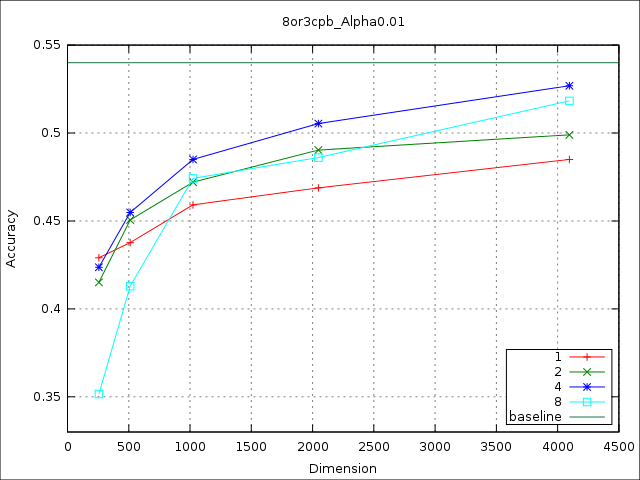
\includegraphics[scale=0.6]{img/resultados/reales/media_8or3cpb_Alpha0,01.png}
				\caption[Reales con umbral media]{Resultado de haber usado la media para el calculo del umbral. La mejor clasificación se logra con los siguientes parámetros: \textit{alpha:0.01}, \textit{bits por grupo: 4}, \textit{dim del vector: 4096}, \textit{orientaciones: 8}, \textit{celdas por bloque: 9}.}
				\label{fig: Reales-media-8or9cpbAlph0.01}
			\end{figure}
			
			\begin{figure}[htbp]
				\centering
				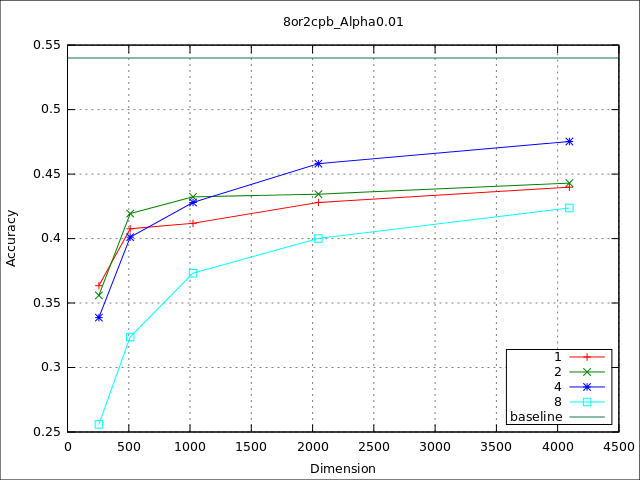
\includegraphics[scale=0.6]{img/resultados/reales/median_8or2cpb_Alpha0,01.png}
				\caption[Reales con umbral mediana]{Resultado de haber usado la mediana para el calculo del umbral. La mejor clasificación se logra con los siguientes parámetros: \textit{alpha:0.01}, \textit{bits por grupo: 4}, \textit{dim del vector: 4096}, \textit{orientaciones: 8}, \textit{celdas por bloque: 4}.}
				\label{fig: Reales-mediana-8or4cpbAlph0.01}
			\end{figure}
			
			\begin{figure}[htbp]
				\centering
				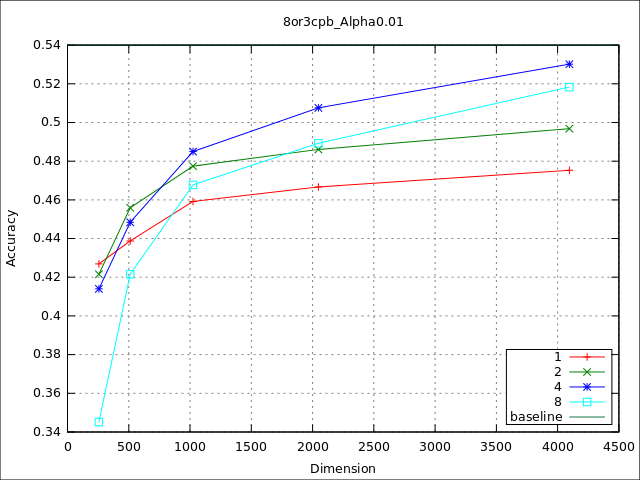
\includegraphics[scale=0.6]{img/resultados/reales/expon_8or3cpb_Alpha0,01.png}
				\caption[Reales con umbral exponencial]{Resultado de haber usado la distribución exponencial para el calculo del umbral. La mejor clasificación se logra con los siguientes parámetros: \textit{alpha:0.01}, \textit{bits por grupo: 4}, \textit{dim del vector: 4096}, \textit{orientaciones: 8}, \textit{celdas por bloque: 9}.}
				\label{fig: Reales-expon-8or9cpbAlph0.01}
			\end{figure}
			
			\begin{figure}[htbp]
				\centering
				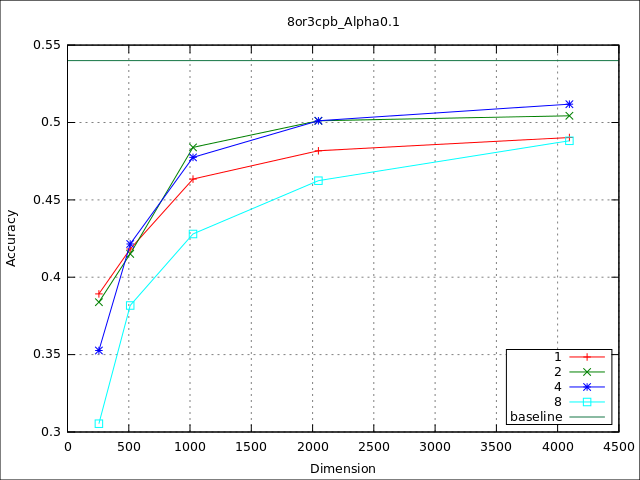
\includegraphics[scale=0.6]{img/resultados/reales/bootstrap_8or3cpb_Alpha0,1.png}
				\caption[Reales con umbral boostrap]{Resultado de haber usado bootstrap para el calculo del umbral. La mejor clasificación se logra con los siguientes parámetros: \textit{alpha:0.1}, \textit{bits por grupo: 4}, \textit{dim del vector: 4096}, \textit{orientaciones: 8}, \textit{celdas por bloque: 9}.}
				\label{fig: Reales-bootstrap-8or9cpbAlph0.1}
			\end{figure}
			
		Después de presentar estos gráficos aclaro que los siguientes experimentos se realizaron utilizando la mejor configuración observada (8 orientaciones, 9 grupos por bloque). Comparación final con los resultados de Wang.
	\begin{table}
		\centering
		\begin{tabular}{ | l | l | l | p{5cm} |}
    			\hline
    				\textbf{NATIVE + FERNS} & \textbf{Score} \\ \hline
    				Wang et al. & 0.54\% \\ \hline
    				Media & 0.53\% \\ \hline
    				Mediana & 0.47\%\\ \hline
    				Exponencial & 0.53\% \\ \hline
    				Bootstrap & 0.51\%\\ 
    			\hline
    		\end{tabular}
    		\caption{Tabla comparativa entre el resultado obtenido por Wang para imágenes naturales y los obtenidos en el presente trabajo, utilizando los cuatro umbrales propuestos.}
    	\end{table}
    	
    	Teniendo en cuenta el resultado de Wang para las imágenes sintéticas, paso a mostrar 
los resultados de haber ido incrementando la proporcion de muestras sintéticas al momento de entrenar al clasificador.

			\begin{figure}[htbp]
				\centering
				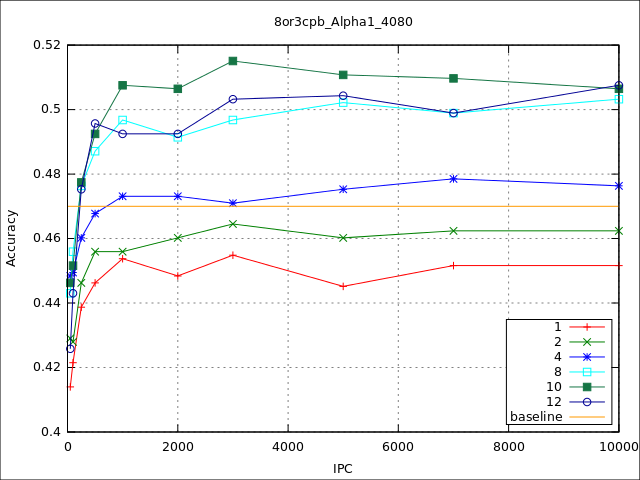
\includegraphics[scale=0.6]{img/resultados/sinteticas/best_media_8or3cpb_Alpha1_4080.png}
				\caption[Sintéticas media bajo resultado]{}
				\label{fig: Sinteticas-media-bajo}
			\end{figure}
			
			\begin{figure}[htbp]
				\centering
				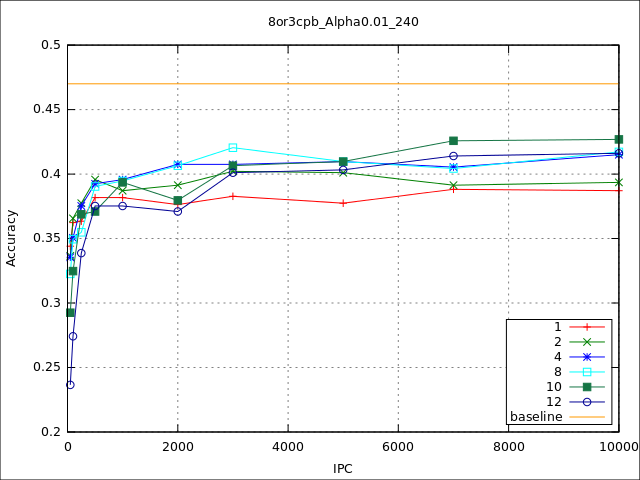
\includegraphics[scale=0.6]{img/resultados/sinteticas/worst_media_8or3cpb_Alpha0,01_240.png}
				\caption[Sintéticas media mejor resultado]{}
				\label{fig: Sinteticas-media-mejor}
			\end{figure}
			
			\begin{figure}[htbp]
				\centering
				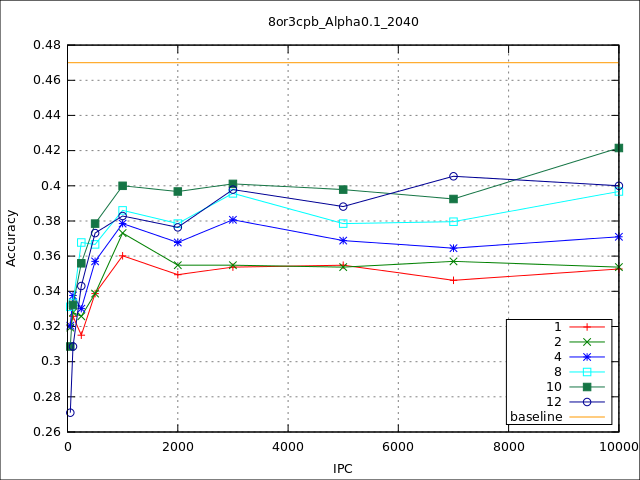
\includegraphics[scale=0.6]{img/resultados/sinteticas/best_median_8or3cpb_Alpha0,1_2040.png}
				\caption[Sintéticas mediana mejor resultado]{}
				\label{fig: Sinteticas-median-mejor}
			\end{figure}
	
			\begin{figure}[htbp]
				\centering
				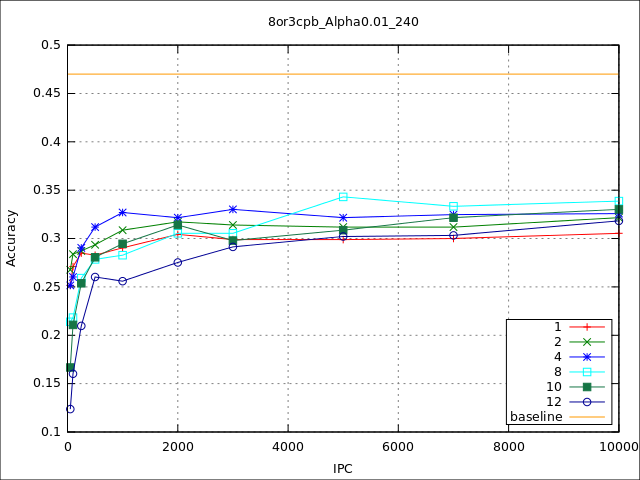
\includegraphics[scale=0.6]{img/resultados/sinteticas/worst_median_8or3cpb_Alpha0,01_240.png}
				\caption[Sintéticas mediana peor resultado]{}
				\label{fig: Sinteticas-median-bajo}
			\end{figure}
				
			\begin{figure}[htbp]
				\centering
				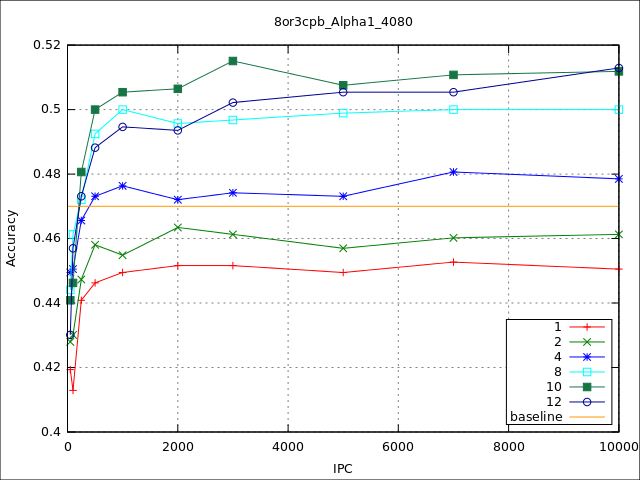
\includegraphics[scale=0.6]{img/resultados/sinteticas/best_expon_8or3cpb_Alpha1_4080.png}
				\caption[Sintéticas exponencial mejor resultado]{}
				\label{fig: Sinteticas-expon-mejor}
			\end{figure}
	
			\begin{figure}[htbp]
				\centering
				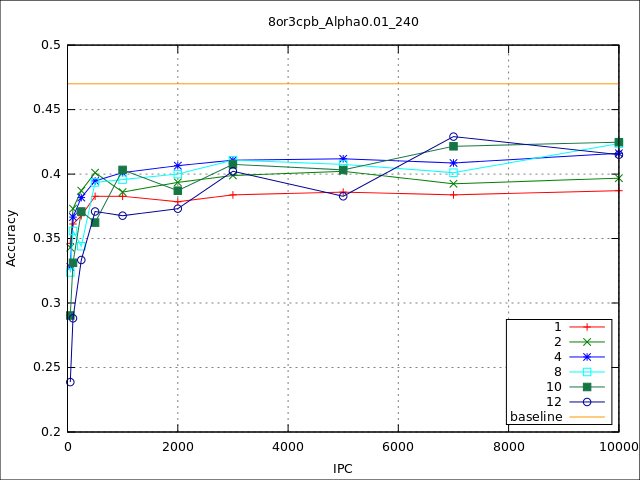
\includegraphics[scale=0.6]{img/resultados/sinteticas/worst_expon_8or3cpb_Alpha0,01_240.png}
				\caption[Sintéticas exponencial peor resultado]{}
				\label{fig: Sinteticas-expon-bajo}
			\end{figure}
			
			\begin{figure}[htbp]
				\centering
				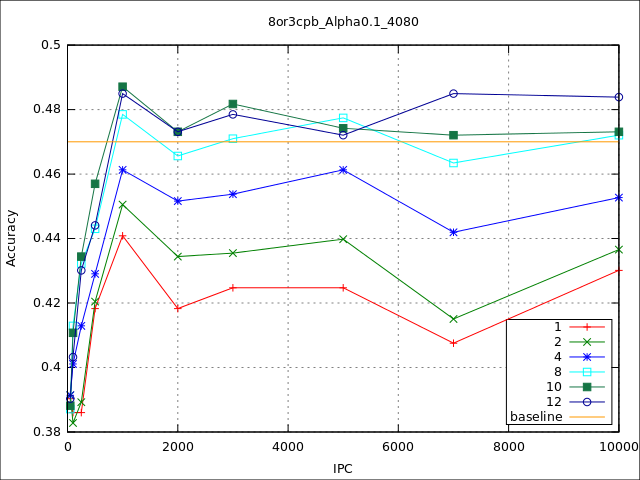
\includegraphics[scale=0.6]{img/resultados/sinteticas/best_bootstrap_8or3cpb_Alpha0,1_4080.png}
				\caption[Sintéticas bootstrap mejor resultado]{}
				\label{fig: Sinteticas-bootstrap-mejor}
			\end{figure}
	
			\begin{figure}[htbp]
				\centering
				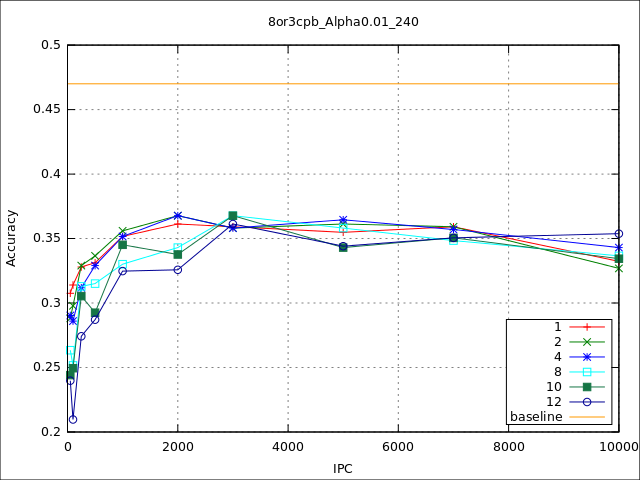
\includegraphics[scale=0.6]{img/resultados/sinteticas/worst_bootstrap_8or3cpb_Alpha0,01_240.png}
				\caption[Sintéticas bootstrap peor resultado]{}
				\label{fig: Sinteticas-bootstrap-bajo}
			\end{figure}

	\newpage
\subsection{Análisis}
	Análisis / discusión
	\begin{itemize}
		\item Comparar la performance al usar diferentes datasets (comparar cantidad de imágenes por clase al usar caracteres sintéticos). Hacer una tabla.
		\item Observaciones sobre errores de clasificación. El problema que surge con algunos caracteres donde no se puede distinguir minúscula de mayúscula con lo cual se producen errores. Mostrar la matriz de confusión del mejor caso donde no se distingan mayúsculas de minúsculas. Otro error donde ciertos caracteres como la "l" se confunden con otros caracteres como el "1".
		\item Comparar en los resultados con los obtenidos por Wang et al. en condiciones similares. Básicamente explicar algo que no explican en su trabajo Wang et al. y que es la influencia en la cantidad de muestras sintéticas por clase.
		\item Análisis de como aumenta la performance de clasificación el mezclar imágenes sintéticas y reales. Mostrar como a medida que aumentamos demasiado la proporción de img. sintéticas, se tiende a disminuir la precisión. Básicamente, la precisión baja para "igualarse" a la precisión obtenida cuando se entrena al clasif con puras imagenes sintéticas (usando la misma cant. de img. por clase).
	\end{itemize}


	%\subsection{Implementación}

	\begin{itemize}
		\item Explicar porque uso python + las librerías involucradas.
		\item Porque uso JSON y no MySQL para almacenar datos.
		\item Datasets usados y su creación.
		\item Pipeline implementado desde la creación del dataset hasta la obtención de resultados del clasificador Random Ferns.
	\end{itemize}

	



	\newpage
\section{Conclusiones y trabajos futuros}

	Para concluir con este trabajo y en base a los resultados expuestos, se puede concluir que la tarea de reconocimiento de caracteres en imágenes estructuradas no es una tarea sencilla. Actualmente han habido bastantes avances en el campo pero todavía no  se logra desarrollar un método que compita con los clasificadores de documentos escaneados.
	
	Basados en los análisis del capítulo 4, se pudo observar que el uso de imágenes sintéticas proporcionó mejoras al momento de entrenar al clasificador si se las combina con imágenes reales. Si bien la mejora no es muy notoria, se puede seguir trabajando para mejorar esto y así poder evitar a futuro el tedioso trabajo de tener que recolectar imágenes. El uso de Random Ferns como clasificador es una buena opción por lo expuesto en el capítulo 2; sin embargo, sería interesante probar con otros para poder realizar una mejor comparación.
	
	Sin duda alguna el desafio de reconocer texto en escenas naturales es un problema que vale la pena estudiar y pulir ya que las aplicaciones que tiene actualmente son enormes. Más aún con la proliferación de los dispositivos móviles y la necesidad de crear aplicaciones que asistan a usuarios con deficiencia visual entre otros.

	\newpage	
\addcontentsline{toc}{section}{Referencias}		% sino no figura en el TOC

\begin{thebibliography}{100}

	\bibitem{wang}
 	 	Kai Wang, Boris Babenko and Serge Belongie,
	 	\emph{``End-to-End Scene Text Recognition''},
		IEEE International Conference on Computer Vision (ICCV), 
		Barcelona, España,
		2011.
		
	\bibitem{WB10}
 	 	Kai Wang and Serge Belongie,
	 	\emph{``Word spotting in the wild''},
		In ECCV, 2010.
		
	\bibitem{fischler}
 	 	M.A. Fischler and R.A. Elschlager,
	 	\emph{``The representation and matching of pictorial
structures''},
		IEEE Transactions on Computer, 
		22(1):67–92,
		Enero 1973.
		
	\bibitem{Bis07}
		Christopher M. Bishop.
		\emph{``Pattern Recognition and Machine Learning (Information Science and Statistics)''}.
		Springer, Octubre 2007.
		
	\bibitem{dCBV09}
		T. E. de Campos, B. R. Babu, and M. Varma.
		Character recognition in natural images.
		In \emph{``Proceedings of the International Conference on Computer Vision Theory and Applications, Lisbon, Portugal,''}
		February, 2009.
		
	\bibitem{KGK^{+}07}
		Sunil Kumar, Rajat Gupta, Nitin Khanna, Santanu Chaudhury, and Shiv Dutt Joshi.
		\emph{``Text extraction and document image segmentation using matched wavelets and mrf model.''}
		\textit{IEEE Transactions on Image Processing}, 16(8):2117-2128, 2007.
	
	\bibitem{DT05}
		Navneet Dalal \& Bill Triggs.
		\emph{``Histograms of oriented gradients for human detection.''}
		In Cordelia Schmid, Stefano Soatto, and Carlo Tomasi, editors, \textit{International Conference on Computer Vision \& Pattern Recognition}, volume 2, pages 886-893, INRIA Rh\^{o}ne-Alpes, ZIRST-655, av. de l'Europe, Montbonnot-38334, June 2005.
		
	\bibitem{PSH2011}
		J. Pradeep, E. Shrinivasan \& S. Himavathi,
		\emph{``Diagonal Based Feature Extraction for Handwritten Alphabets Recognition System Using Neural Network''},
		International Journal of Computer Science \& Information Technology(IJCSIT),
		vol.3, No 1, February 2011.
		
	\bibitem{Suen86}
		C. Y. Suen,
		\emph{``Character recognition by computer and applications''},
		in Handbook of Patter Recognition and Image Processing,
		New York: Academic,
		pp. 569-586,
		1986

		
	\bibitem{Heutte98}
		L. Heutte, T. Paquet, J. V. Moreau, Y. Lecourtier and C. Olivier,
		\emph{``Structural/statistical feature based vector for handwritten character recognition''},
		Pattern Recognition Letters,
		Vol. 19(7), pp. 629-641,
		1998.
		
	\bibitem{Hussain72}
		A. B. S. Hussain, G. T. Toussaint and R. W. Donaldson,
		\emph{``Results obtained using a simple character recognition procedure on Munson’s handprinted data''},
		IEEE Transactions on Computers, pp. 201-205,
		1972.
		
	\bibitem{Glauberman56}
		M. H. Glauberman,
		\emph{``Character recognition for business
machines''},
		Electronics,
		Vol. 29, pp. 132-136,
		1956.
		
	\bibitem{TR93}
		R. Tarling and R. Rohwer,
		\emph{``Efficient use of training data in
the n-tuple recognition method''},
		Electronics Letters,
		Vol. 29(24), pp. 2093-2094,
		1993
		
	\bibitem{RP94}
		J. Rocha and T. Pavlidis,
		\emph{``A shape analysis model with applications to a character recognition system''},
		IEEE Transactions on PAMI,
		Vol. 16(4), pp. 393-404, 
		1994.
		
	\bibitem{Amin2000}
		A. Amin,
		\emph{``Recognition of printed Arabic text based on global features and decision tree learning techniques''},
		\textit{Patter Recognition},
		Vol. 33, pp. 1309-1323,
		2000.
	
	\bibitem{NNSJ}
		Nadira Muda, Nik Kamariah, Nik Ismail, Siti Azami Abu Bakar, Jasni Mohamad Zain,
		\emph{``Optical Character Recognition By Using Template Matching(Alphabet)''},
		Universiti Malaysia Pahang.
		
	\bibitem{SA96}
		S. Lucas, A. Amiri
		\emph{``Statistical Syntactic Methods for High Performance OCR''}
		Vision, Image and Signal Processing, IEE Proccedings,
		vol. 134, Issue 1, pp. 23-30,
		February 1996.
		
	\bibitem{RYVY2010}
		Raghuraj Singh, C. S. Yadav, Prabhat Verma, Vibhash Yadav,
		\emph{``Optical Character Recognition (OCR) for Printed Devnagari Script Using Artificial Neural Network''},
		International Journal of Computer Science \& Communication,
		January-June  2010.
	
	\bibitem{Eikvil}
		Line Eikvil.
		\emph{``Optical Character Recognition''}.
		\url{http://www.nr.no/~eikvil/OCR.pdf}.
		December, 1993.
		
	\bibitem{GKurt}
		Dr. Gordon Kurtenbach (2010).
		\emph{``Pen-Based Computing''}.
		\emph{XRDS}, vol.16, num.4, pp.14-20.
		Obtenido de \url{http://www.autodeskresearch.com/pdf/penbasedcomputing-kurtenbach.pdf}.
		
	\bibitem{x-root}
		Andor Grei{\ss}l.(2009).
		\emph{Cardreader}(v2.0.10)[Mobile Application Software].
		Obtenido de \url{https://itunes.apple.com/de/app/id333992036?mt=8}
		
	\bibitem{arh-anpr}
		ARH Inc.
		\emph{The CARMEN\textregistered Parking ANPR Software}[Computer Software].
		Obtenido de \url{http://www.anpr.net/anpr_09/anpr_parking.html}
		
	\bibitem{arh-passport}
		ARH Inc.
		\emph{PRM(Passport Reader Multireader)}[Computer Device].
		Obtenido de \url{http://www.passport-reader.com/prm_passport_reader.html}
		
	\bibitem{arh-card}
		ARH Inc.
		\emph{Card Reader}[Computer Device].
		Obtenido de \url{http://www.passport-reader.com/card_reader.html}
	
	\bibitem{creaceed}
		Creaceed S.P.R.L (2010).
		\emph{Prizmo}(v3.1.5)[Mobile Application Software].
		Obtenido de \url{https://itunes.apple.com/gb/app/prizmo-scanning-ocr-speech/id366791896?mt=8}
		
	\bibitem{sunnyside}
		SUNNYSIDESOFT (2013).
		\emph{VirtualTablet Lite (S-Pen)}(v1.2)[Mobile Application Software].
		Obtenido de \url{https://play.google.com/store/apps/details?id=com.sunnysidesoft.VirtualTablet}
		
	\bibitem{gbook}
		Google Inc.(2004).
		\emph{Google Books}[Web Service].
		Obtenido de \url{http://books.google.com/}.
		
	\bibitem{Tauschek}
		G. Tauschek,
		\emph{``Reading Machine''},
		U.S. Patent 2026329,
		December 1935.
		
	\bibitem{Handel}
		P. W. Handel,
		\emph{``Statistical machine''}
		U.S. Patent 1915993,
		June 1933.
	
	\bibitem{Tesseract}
		Google Inc.(2005).
		\emph{``Tesseract''}
		Obtenido de \url{https://code.google.com/p/tesseract-ocr/}
		
	\bibitem{YoutubeStats}
	Google Inc.
	\emph{``Youtube statistics''}.
	Obtenido de \url{http://www.youtube.com/yt/press/es/statistics.html}
	
	\bibitem{Websites}
	Google Inc. 
	Official Blog.
	Obtenido de \url{http://googleblog.blogspot.com.ar/2008/07/we-knew-web-was-big.html}
	
	\bibitem{GoogleSearches}
	Statistic Brain.
	\emph{``Google Annual Search Statistics''}(2014).
	Obtenido de \url{http://www.statisticbrain.com/google-searches/}
	
	\bibitem{DP97}
		Domingos, P. y M. Pazzani (1997).
		\emph{``On the optimality of the simple bayesian classifier under zero-one loss''}. \textit{Machine Learning} 29, pp. 103-130.
		
	\bibitem{SpamPaper}
		T. S. Guzella, W. M. Caminhas.
		\emph{``A review of machine learning approaches to Spam filtering''}.
		Expert Systems with Applications.
		2009.
		
	\bibitem{BrownLowe07}
		Brown, M. and Lowe, D. (2007).
		\emph{``Automatic panoramic image stitching using invariant features''}.
		\textit{International Journal of Computer Vision},
		74(1):59–73.
	
	\bibitem{FPZ07}
		Fergus, R., Perona, P., and Zisserman, A. (2007).
		\emph{``Weakly supervised scale-invariant learning of models for visual recognition''}.
		\textit{International Journal of Computer Vision},
		71(3):273–303.
		
	\bibitem{Breiman01}
		Breiman, L.
		\emph{``Random Forests''}.
		Machine Learning 45(1), 5-32.
		January 2001.
		
				
	\bibitem{HOGImages}
		Levi G., (2013, August 18).
		\emph{``A Short introduction to descriptors''}[blog post].
		Obtenido de \url{http://gilscvblog.wordpress.com/2013/08/18/a-short-introduction-to-descriptors/}.
	
	\bibitem{Ozuysal}
		Ozuysal, M., Calonder, M., Lepetit, V. \& Fua, P.
		\emph{``Fast Keypoint Recognition using Random Ferns''}.
		IEEE Transactions on Pattern Analysis and Machine Intelligence,
		32, 448-461 (2010)
		
	\bibitem{DAB}
		Donoser, M., Arth, C. \& Bischof, H.
		\emph{``Detecting, Tracking and Recognizing License Plates''}.
		Institute for Computer Graphic and Vision.
		
	\bibitem{Nadejda}
		Nadejda S. Roubtsova , Rob G.J. Wijnhoven and Peter H.N. de With.
		\emph{``Integrated Text Detection and Recognition in Natural Images''}.
		
	\bibitem{LoweDavid04}
		Lowe, David G. (2004).
		\emph{``Distinctive Image Features from Scale-Invariant Keypoints''}.
		\textit{International Journal of Computer Vision.}
		
	\bibitem{LoweDavid99}
		Lowe, David G. (1999).
		\emph{``Object recognition from local scale-invariant features''}.
		Proceedings of the International Conference on Computer Vision 2.
		pp. 1150–1157.
		
	\bibitem{SJC08}
		J. Shotton, M. Johnson, and R. Cipolla.
		\emph{``Semantic texton forests for image categorization and segmentation''}.
		In \textit{CVPR}, 2008.
		
	\bibitem{OFL07}
		M. Ozuysal, P. Fua, and V. Lepetit.
		\emph{``Fast keypoint recognition in ten lines of code''}.
		In \textit{CVPR}, 2007.
		
	\bibitem{QuinlanID3}
		J. R. Quinlan.
		\emph{``Induction of Decision Trees''}.
		Machine Learning 1: 81-106.
		March 1986.
		
	\bibitem{QuinlanC45}
		J. R. Quinlan.
		\emph{``C4.5: Programs for Machine Learning''}.
		Morgan Kaufmann Publishers, 1993.
		
	\bibitem{PDomingo}
		P. Domingo.
		\emph{``A Few Useful Things to Know about Machine Learning''}.
		Department of Computer Science and Engineering.
		University of Washington.
		
	\bibitem{GPP03}
		B. Gatos, I. Pratikakis and S. Perantonis.
		\emph{``Towards Text Recognition in Natural Scene Images''}.
		Computational Intelligence Laboratory, Institute of Informatics and Telecommunications.
		
	\bibitem{LNJM}
		L. Neumann and J. Matas.
		\emph{``Real-Time Scene Text Localization and Recognition''}.
		In \textit{CVPR}, 2012.
		
	\bibitem{PiotrD}
		Piotr Dollár.
		\emph{``Piotr's Image and Video Matlab Toolbox (PMT)''}.
		Obtenido de \url{http://vision.ucsd.edu/~pdollar/toolbox/doc/index.html}. 
		
	\bibitem{LBreiman96}
		L. Breiman.
		\emph{``Bagging Predictors''}.
		Septiembre 1994.
		
	\bibitem{WordLens}
		Quest Visual.
		\emph{``Word Lens''}(2014).
		Obtenido de \url{http://questvisual.com/}

	\bibitem{Optelec}
		Optelec.
		\emph{``Optelec ClearReader+''}(2014).
		Obtenido de \url{http://us.optelec.com/products/crbaus-optelec-clearreader.html}	
		
	\bibitem{GargRo01}
		A. Garg and D. Roth.
		\emph{``Understanding Probabilistic Classifiers''}.
		In \textit{EMCL}, 2001.
		
	\bibitem{Murphy12}
		K. P. Murphy. (2012).
		\emph{``Machine Learning A Probabilistic Perspective''}.
		Cambridge: The MIT Press.
				
\end{thebibliography}

	\newpage	
\appendix
	\appendix
\section{Conceptos de probabilidad y notación}

	A continuación se introducirán algunos conceptos de probabilidad que serán de utilidad en el desarrollo de las secciones posteriores.

	\paragraph*{Variables aleatorias discretas} ~\\

		Dado un evento $A$, la expresión $p(A)$ denota la probabilidad de que $A$ sea verdadero. Por ejemplo, $A$ puede ser la expresión lógica ``Va a llover mañana''. Se requiere que $0 \leq p(A) \leq 1$, donde $p(A)=0$ significa que el evento no va a ocurrir, y $p(A)=1$ significa que el evento definitivamente va a suceder. Escribimos $p(\overline{A})$ para denotar la probabilidad del evento no $A$, es decir, de que el evento no ocurra; esto se define como $p(\overline{A})=1-p(A)$. Se escribirá $A=1$ para hacer referencia que el evento $A$ es verdadero, y $A=0$ cuando el evento $A$ es falso.
		
		Se puede extender la noción de eventos binarios definiendo una \textit{variable aleatoria discreta} $X$, la cual puede tomar cualquier valor de un conjunto finito o infinito contable \scalebox{1.4}{$\chi$}. Se denota la probabilidad de que $X=x$ por $p(X=x)$, o sólo $p(x)$ como abreviación. Ambas notaciones se van a usar indistintamente en el desarrollo del trabajo. Aquí $p: x \rightarrow \mathbb{R} $ se denomina \textit{función de probabilidad}. Esta satisface las propiedades $0 \leq p(x) \leq 1$ y $\sum_{x \in \chi}p(x)=1$.
		
	\paragraph*{Probabilidad de la unión de dos eventos} ~\\
		
		Dados dos eventos, $A$ y $B$, se define la probabilidad de A o B de la siguiente manera:
		\begin{align}
			p(A \lor B) &= p(A) + p(B) - p(A \land B) \\
			&= p(A) + p(B) ~\text{si A y B son mutuamente excluyentes}
		\end{align}
		
	\paragraph*{Probabilidad conjunta} ~\\
	
		Se define la probabilidad del evento conjunto A y B como sigue:
		\begin{align}
			p(A,B) = p(A \land B)
		\end{align}

		A esta ecuación se la llama \textit{regla del producto}. Dada la distribución conjunta en dos eventos p(A,B), se define la ``distribución marginal'' de la variable aleatoria $A$ de la siguiente manera:
		\begin{align}
			p(A)=\sum_{b}p(A,B=b)
		\end{align}
		donde se asumen todos los estados posibles de B. Se puede definir p(B) de forma similar. A esta ecuación se la denomina regla de la suma o regla de la probabilidad total.
		
	\paragraph*{Probabilidad condicional} ~\\
	
		Se define la probabilidad condicional del evento A, dado que el evento B es verdadero, como sigue:
		\begin{align}
			p(A|B) = \frac{p(A,B)}{p(B)} ~\text{si}~ p(B)>0
		\end{align}
		
	\paragraph*{Regla de Bayes} ~\\
		
		Combinando la definición de probabilidad condicional con las reglas del producto y la suma se obtiene la \textit{regla de Bayes}, también llamada \textit{Teorema de Bayes}:
		\begin{align}\label{eq:bayes}
			p(X=x|Y=y) &= \frac{p(X=x,Y=y)}{p(Y=y)} \\
			&= \frac{p(X=x)p(Y=y|X=x)}{\sum_{x'}p(X=x')p(Y=y|X=x')}
		\end{align}

	\paragraph*{Independencia e independencia condicional} ~\\
	
		Se dice que $X$ e $Y$ son independientes, denotado como $X \bot Y$	, si se puede representar la unión como el producto de dos marginales, es decir,
	\begin{align}
		X \bot Y \Longleftrightarrow p(X,Y) = p(X)p(Y)
	\end{align}			
			
		En general, se dice que un conjunto de variables es mutuamente independiente si la conjunta puede ser escrita como producto de marginales.
		
		Desafortunadamente, la independencia es rara, porque la mayoría de las variables pueden influir en la mayoría de las otras variables. Sin embargo, usualmente esta influencia se da a través de otras variables en vez de ser directa. Por lo tanto se dice que $X$ e $Y$ son \textit{condicionalmente independientes} dada $Z$ si y solo si la conjunta condicional puede ser escrita como producto de marginales condicionales:
		\begin{align}
			X \bot Y|Z \Longleftrightarrow p(X,Y|Z) = p(X|Z)p(Y|Z)
		\end{align}
	

	
	\section{Gradiente}
\label{section:Apendice-C}

En este apéndice, se busca realizar una introducción básica al concepto de gradiente con el objetivo de poder comprender mejor como funcionan los descriptores HOG.

Sea $f(x_1,\dots,x_n)$ una función escalar de múltiples variables. Como expresa Gonzales et. al. en \cite{GonWoods}, el gradiente de $f$ es un vector que apunta en la dirección donde se registra la mayor tasa de incremento de la función. Su magnitud es la pendiente del gráfico en esa dirección. Es la generalización del concepto de derivada en funciones de múltiples variables.
		
	El gradiente de la función $f$ descrita anteriormente, es denotado como $\nabla f$ donde $\nabla$, el símbolo nabla, denota el operador diferencial. El gradiente de $f$ es definido como el único campo vectorial cuyo producto punto con cualquier vector $v$ en cada punto $x$ es la derivada direccional de $f$ a lo largo de $v$. Es decir,
		 \begin{align*}
		 	(\nabla f(x))\cdot v = D_v f(x)
		 \end{align*}
		 
	En un sistema de coordenadas rectangular, el gradiente es el campo vectorial cuyos componentes son las derivadas parciales de $f$:
		 
		 \begin{align*}
		 	\nabla f(x) = \frac{\partial f}{\partial x_1}\mathbf{e}_1 + \cdots + \frac{\partial f}{\partial x_n }\mathbf{e}_n
		 \end{align*}
	donde los $\mathbf{e}_i$ son vectores unitarios ortogonales que apuntan en la dirección de coordenadas.

	En el procesamiento de imágenes, un gradiente es un cambio direccional en la intensidad o color de la imagen. En \cite{DJacobs}, Jacobs explica que el vector gradiente se forma combinando la derivada parcial de la imagen en las direcciones $x$ e $y$. Se puede expresar de la siguiente forma:
		\begin{align}
			\nabla I = \left( \frac{\partial I}{\partial x} , \frac{\partial I}{\partial y} \right)
		\end{align}	
		
	donde \textit{I}: $\mathbb{R}^{2} \rightarrow [0, 1]$, es la ``función intensidad'' que asigna un valor de intensidad a cada pixel, par (x,y), de la imagen. Según Jacobs, cuando determinamos la derivada parcial de $I$ respecto de $x$, determinamos la rapidez con que la imagen cambia de intensidad a medida que $x$ cambia. Para funciones continuas, $I(x,y)$, podemos expresarlo de la siguiente manera:
	\begin{align}
		\frac{\partial I(x,y)}{\partial x} = \lim_{\nabla x\rightarrow 0} \frac{I(x + \nabla x, y) - I(x,y)}{\nabla x}	
	\end{align}
	
	 El cálculo de los gradientes de una imagen es útil ya que sirve, por ejemplo, para realizar detección de bordes de un objeto. La detección de bordes busca identificar puntos en una imagen en donde el brillo de la misma cambie de manera abrupta o, más formalmente, tenga discontinuidades. El propósito de esto es capturar eventos importantes o cambios en las propiedades de una imagen. En este caso, después de que los gradientes han sido computados, los píxeles con alto valor de gradiente son elegido como posibles bordes. Los píxeles con el valor de gradiente más alto en la dirección del gradiente se convierten en píxeles de borde. Los gradientes, también pueden ser usados en aplicaciones que realizan reconocimiento de objetos o correspondencia de texturas.	 
	
	\section{Sistema Operativo, Hardware y Software}
\label{section:Apendice-B}
	La mayor parte de los algoritmos fueron desarrollados en el Sistema Operativo \textit{Ubuntu (Linux)}. Al haber elegido Python como lenguaje de programación permite utilizarlos en distintas plataformas, como \textit{Mac} y \textit{Windows}, sin problemas.
	
	\subsection{Datos Específicos sobre Hardware Utilizado}
		\textbf{Computadora\footnote{Utilizada solamente para procesar los resultados obtenidos del servidor y generar los gráficos necesarios.}:}
		\begin{itemize}
			\item Procesador: Intel\textregistered ~Core\texttrademark ~i7-4700MQ CPU @ 2.40GHz $\times$ 8 
			\item Memoria Ram: 16 GB 1333 Mhz DDR3
			\item Sistema Operativo: Ubuntu 14.04 LTS x64
		\end{itemize}
		
		\textbf{Servidor ``Ganesh''\footnote{Servidor proporcionado por la \textit{FaMAF} para correr los experimentos.}:}
		\begin{itemize}
			\item Micros: 4xDualCore AMD Opteron\texttrademark ~Processor 8212.
			\item Placa madre: SuperMicro H8QM8.
			\item Memoria Ram: 32 GB DDR2.
			\item Sistema Operativo: Ubuntu 12.04.5 LTS x64. 
		\end{itemize}
				
	\subsection{Datos Específicos sobre Software Utilizado}
		\begin{itemize}
			\item Python Versión 2.7.6
			\item Pillow Versión 2.4.0
			\item GCC Versión 4.8.2
			\item numpy Versión 1.8.1
			\item matplotlib Versión 1.3.1
			\item ipython Versión 2.1.0
			\item ipdb Versión 0.8
			\item git Versión 1.9.1
			\item scikit-image Versión 0.10.0
			\item scipy Versión 0.14.0
		\end{itemize}

	\subsection{Herramientas de Software utilizadas}
	    Durante la realización de la tesis, se usaron varias herramientas \textit{de software libre} que fueron indispensables y de una utilidad crucial. \\
	    \\
	   \textbf{ Algunas de estas herramientas fueron:}
	   \begin{itemize}

	       \item SUBLIME TEXT: IDE que se utilizó para escribir todo el código Python del presente trabajo\footnote{http://www.sublimetext.com/}.
	               	%--> Imagen ''sublime-text_logo.png''
					\begin{figure}[htbp]
						\centering
						\fbox{ 
\includegraphics[scale=0.35]{img/sublime_logo.png} }
						\caption{SUBLIME-TEXT IDE.}
						\label{fig:sublime_ide}
					\end{figure}

	       \item TexMaker: IDE que se usó para escribir todo el código \LaTeX{} de la tesis\footnote{http://www.xm1math.net/texmaker/}.
	               	%--> Imagen ''texmaker_logo.png''
					\begin{figure}[htbp]
						\centering
						\fbox{ 
\includegraphics[scale=1]{img/texmaker_logo.png} }
						\caption{Texmaker.}
						\label{fig:texmaker}
					\end{figure}
das
	       \item GIT: Sistema de control de versiones usado para todo el código\footnote{http://git-scm.com/}.
	               	%--> Imagen ''git_logo.png''
					\begin{figure}[htbp]
						\centering
						\fbox{ 
\includegraphics[scale=1]{img/git_logo.png} }
						\caption{GIT.}
						\label{fig:git}
					\end{figure}
	   \end{itemize}
	
	\subsection{Por qué Python?}	
	
	El lenguaje que se ha elegido para programar al clasificador como así también todos los módulos de procesamiento de resultados es Python. Las razones por las cuales se elige este lenguaje y no otro son muchas, entre las cuales algunas de las más importantes son:
	
			\begin{itemize}
	
			\item Python tiene una comunidad muy activa y cooperativa: La comunidad de programadores que programan con Python es muy grande (y tiende a seguir creciendo), y se caracteriza fuertemente por una muy buena aceptación de nuevos miembros y una gran predisposición a la ayuda mutua en medios como foros y listas de correos, como la lista de correo de PyAr (Python Argentina). Esto muestra que Python es un lenguaje vivo y en crecimiento.
			
			\item Python es un lenguaje con una sintaxis sencilla y es fácil de entender y aprender.
			
			\item Python es rápido: Python cuenta con una enorme cantidad de librerías magníficas implementadas en C (como NumPy o SciPy) que permiten realizar operaciones complejas en cuanto a procesamiento de manera sumamente rápida y eficiente. Incluso si no existiera una librería en particular en C para la funcionalidad que se desea, se puede implementar la porción de código que realiza la función crítica en C y utilizarla desde Python.
			
			\item Python tiene un gran soporte para computación científica: con librerías sólidas, fuertemente mantenidas, bien documentadas y áltamente eficientes, como SciPy, NumPy, matplotlib, entre otros.
			
			\item Python es multiplataforma: el código Python de este trabajo podrá ser utilizado prácticamente en cualquier sistema operativo. Esto es una ventaja importantísima y no limita al usuario a un sistema operativo o hardware en particular.
			\end{itemize}

	


	%\newpage
Córdoba, Argentina, 2014\\[9.5cm]
\begin{flushright}
    \textit{Rodrigo Carranza Astrada}
\end{flushright}


\end{document}
